% Last update/Última versão: 11/Sep/2016
%%%%%%%%%%%%%%%%%%%%%%%%%%%%%%%%%%%%%%%%%%%%%%%%%%%%%%%%%%%%%%%%%%%%%%
%=====================================================================
% 							Pacotes Fundamentais
%=====================================================================
\documentclass[
% -- op\c{c}\~{o}es da classe memoir --
12pt,				% tamanho da fonte
oneside,			% para impress\~{a}o em verso e anverso. Oposto a oneside
a4paper,		% tamanho do papel.
% -- op\c{c}\~{o}es da classe abntex2 --
%chapter=TITLE,		% t\'{\i}tulos de cap\'{\i}tulos convertidos em letras mai\'{u}sculas
%section=TITLE,		% t\'{\i}tulos de se\c{c}\~{o}es convertidos em letras mai\'{u}sculas
%subsection=TITLE,	% t\'{\i}tulos de subse\c{c}\~{o}es convertidos em letras mai\'{u}sculas
%subsubsection=TITLE,% t\'{\i}tulos de subsubse\c{c}\~{o}es convertidos em letras mai\'{u}sculas
% -- op\c{c}\~{o}es do pacote babel --
english,			% idioma adicional para hifeniza\c{c}\~{a}o
%french,			% idioma adicional para hifeniza\c{c}\~{a}o
%spanish,			% idioma adicional para hifeniza\c{c}\~{a}o
brazil,				% o \'{u}ltimo idioma \'{e} o principal do documento
%sumario=tradicional,
]{article}
\usepackage[a4paper, 
right = 1.5cm, left = 2cm, top = 1.5cm, bottom = 2cm]{geometry}
\usepackage[utf8]{inputenc}
\usepackage[english,portuguese]{babel}
%\usepackage[myheadings]{fullpage}
\usepackage[T1]{fontenc}
\usepackage{indentfirst}
\usepackage{graphicx, setspace}
\usepackage{booktabs}
\usepackage{sectsty}
\usepackage{url}
\usepackage{times}    %similar to \usepackage{mathptm}
\usepackage{comment}
\usepackage{multirow}
\usepackage{graphicx}
\usepackage[table,xcdraw]{xcolor}
\usepackage{enumitem}
\usepackage{blindtext}
\usepackage{float}
\usepackage[bottom]{footmisc}
\usepackage{pdfpages}
\usepackage{caption} % \caption*
\usepackage{csquotes}
\usepackage{footnote} % Permite footnote em tabelas
\usepackage{titlesec}


%=====================================================================
% 							Pacotes Bibliográficos
%=====================================================================
\usepackage[backend=biber,
	style = abnt,%
	noslsn, %
	extrayear, %
	uniquename=init,% 
	giveninits, %
	justify, %
	sccite,% 
	scbib, %
	repeattitles, %
	doi=false,isbn=false,url=false, 
	maxcitenames=2 % Não consegui deixar et al em itálico
	]{biblatex}
\addbibresource{./refs.bib}
\AtEveryBibitem{%clear month
  \clearfield{labelmonth}
  \clearfield{labellanguage}
}


\makeatletter %%%% \textcites
\renewbibmacro*{cite:init}{%
  \ifnumless{\value{multicitecount}}{2}%
    {\global\boolfalse{cbx:parens}%
     \global\undef\cbx@lasthash%
     \global\undef\cbx@lastyear}%
    {}}%
\makeatother
%%%%%%%%%%%%%%%%% https://tex.stackexchange.com/questions/142999/the-proper-way-to-cite-the-earliest-publication-date-in-brackets-followed-by
\DeclareLabeldate{%
  \field{date}
  \field{year}
  \field{eventdate}
  \field{urldate}
  \literal{nodate}
}

\renewbibmacro*{date+extradate}{%
  \iffieldundef{labelyear}
    {}
    {\printtext[parens]{%
       \iffieldundef{origyear}
         {}
         {\printtext[brackets]{\printorigdate}%
          \setunit{\addspace}}%
       \iflabeldateisdate
         {\printdateextra}
         {\printlabeldateextra}}}}

\renewbibmacro*{cite:labeldate+extradate}{%
  \iffieldundef{labelyear}
    {}
    {\printtext[bibhyperref]{%
       \iffieldundef{origyear}
         {}
         {\printtext[brackets]{\printorigdate}%
          \setunit{\addspace}}%
       \printlabeldateextra}}}

\renewenvironment{quote}
{\small\list{}{\fontsize{10pt}{12pt}\singlespacing\rightmargin=0cm \leftmargin=4cm}%
	\item\relax}
{\endlist}

%=====================================================================
% 							Comandos específicos da FAPESP
%=====================================================================
%=========================================================================
 %                             Novos Comandos
 %=========================================================================
\newcommand{\HRule}[1]{\rule{\linewidth}{#1}}
\onehalfspacing
\setcounter{tocdepth}{3}
\setcounter{secnumdepth}{3}

\newcommand{\titulo}[1]{\def\meuTitulo{#1}}
\newcommand{\tituloIngles}[1]{\def\meuTituloIngles{#1}}
\newcommand{\numFAPESP}[1]{\def\numFAP{#1}}
\newcommand{\tipoRelatorio}[1]{\def\tipoRelat{#1 }} %o espaço depois do #1 é importante
\newcommand{\autor}[1]{\def\nomeAutor{#1}}
\newcommand{\cidade}[1]{\def\nomeCidade{#1}}
\newcommand{\universidade}[1]{\def\nomeUniversidade{#1}}
\newcommand{\faculdade}[1]{\def\nomeFaculdade{#1}}
\newcommand{\periodoVigencia}[1]{\def\periodVig{#1}}
\newcommand{\periodoRelatorio}[1]{\def\periodRelat{#1}}
\author{Gabriel Petrini da Silveira}
\date{Julho de 2018}

\newcommand{\Figure}[1]{Figura~\ref{fig:#1}}
\newcommand{\Table}[1] {Tabela~\ref{#1}}
\newcommand{\Equation}[1] {Equa\c{c}\~ao~\ref{#1}}
\newcommand{\addFigure}[3] { %Parametros scale, fig_name, caption 
    \begin{figure}[!hbt]
      \centering
      \includegraphics[scale=#1]{figures/#2}
      \caption{#3}\label{fig:#2}
    \end{figure}
}

%=========================================================================
 %                             Capa-Título
 %=========================================================================

\newcommand{\geraTitulo}{
\clearpage
\begin{titlepage}
  \begin{center}
      \vspace*{-3cm}
      { \setstretch{.5} 
        \textsc{\nomeUniversidade} \\
        \HRule{.2pt}\\
        \textsc{\nomeFaculdade}
      }

      \vspace{5.5cm}

      \Large \textbf{\textsc{\meuTitulo}}
	  \HRule{1.5pt} \\ [0.5cm]
      \linespread{1}
      \large Projeto de Pesquisa para Solicitação  de Auxílio à Pesquisa Regular na modalidade Mestrado, fomentado pela Fundação de Amparo à Pesquisa do Estado de São Paulo. \\ 
  	   \HRule{1.5pt} \\ [0.5cm]
%       Projeto FAPESP \texttt{\#\numFAP}
       
       Candidato: \nomeAutor
         \\ [0.1cm]
       Orientador: Lucas Azeredo da Silva Teixeira
       \\ [0.1cm]
       %Co-orientador: Franklin Leon Perez Serrano
       \vfill
       {\normalsize  \nomeCidade, Julho de 2018}
\end{center}
\end{titlepage}
}
%=========================================================================
 %                             Fonte-Headings
 %=========================================================================
\usepackage{titlesec}
\titleformat{\chapter}{\normalfont\LARGE\bfseries}{\thechapter}{1em}{}
\titlespacing*{\chapter}{0pt}{3.5ex plus 1ex minus .2ex}{2.3ex plus .2ex}
\newcommand{\chapterbreak}{\let\clearpage\relax}

\addto\captionsportuguese{\renewcommand{\contentsname}{Sumário}}
\addto\captionsportuguese{\renewcommand{\bibname}{Referências bibliográficas}}

%=========================================================================
 %                             Resumo e Abstract
 %=========================================================================
\newcommand{\Resumo}[1]{
   \begin{otherlanguage}{portuguese}
       \begin{abstract} \thispagestyle{plain} \setcounter{page}{2}
          #1
        \end{abstract}
   \end{otherlanguage} 
} %end \Resumo


\newcommand{\Abstract}[1]{
   \begin{otherlanguage}{english}
      \begin{abstract} \thispagestyle{plain} \setcounter{page}{3}
       #1
      \end{abstract}    
    \end{otherlanguage} 
} %end \abstract

%=========================================================================
 %                             Folha de rosto
 %=========================================================================

%=========================================================================
 %                             Informações gerais do projeto
 %=========================================================================
%INFORMAÇÕES GERAIS DO PROJETO. Não é necessário para uma proposta de projeto

\newcommand{\folhaDeRosto}{
   \section*{Informações Gerais do Projeto}
   \begin{itemize}
      \item Título do projeto: 
            \begin{itemize}\item[] \textbf{\meuTitulo} \end{itemize}
      \item Nome do candidato: 
            \begin{itemize}\item[]\textbf{\nomeAutor}\end{itemize}
      \item Nome do orientador:
                  \begin{itemize}\item[]\textbf{Lucas Azeredo da Silva Teixeira}\end{itemize}
      \item Instituição sede do projeto: 
            \begin{itemize}
               \item[]\textbf{\nomeFaculdade \ da \nomeUniversidade} 
            \end{itemize}
   \end{itemize}
}

\newcommand{\folhaDeRostoEN}{
	\clearpage
	\section*{General project information}
	\begin{itemize}
		\item Project title: 
		\begin{itemize}\item[] \textbf{\meuTitulo} \end{itemize}
		\item Applicant's Name: 
		\begin{itemize}\item[]\textbf{\nomeAutor}\end{itemize}
		\item Supervisor's Name:
		\begin{itemize}\item[]\textbf{Lucas Azeredo da Silva Teixeira}\end{itemize}
		\item Project Institution: 
		\begin{itemize}
			\item[]\textbf{\nomeFaculdade \ da \nomeUniversidade} 
		\end{itemize}
	\end{itemize}
}
%=====================================================================
% 							Outros Pacotes
%=====================================================================
\usepackage{subfigure}
\usepackage{setspace}
\usepackage{lipsum}  
\usepackage{amsmath} % Para cases
\usepackage[cm]{fullpage}
%\usepackage[medium,compact]{titlesec}

%=====================================================================
% 							Página de título e folha de rosto
%=====================================================================
%-----
% Página de título
% Observação: As definições que aparecem a seguir comporão a
%             página de título e a folha de rosto.
%-----
%% Define o nome da universidade onde o projeto foi desenvolvido.
\universidade{Universidade Estadual de Campinas}
%
%% Define o nome da faculdade onde o projeto foi desenvolvido.
\faculdade{Instituto de Economia}
%
%% Define o título do projeto.
\titulo{Título}
%
%
%% Define o autor do relatório.
\autor{}
\cidade{Campinas}


\begin{document}
%=====================================================================
% 							Numeração pré-textual
%=====================================================================
\pagenumbering{roman}
%=====================================================================
% 							Folha de título
%=====================================================================
%\geraTitulo
%=====================================================================
% 							Folha de rosto
%=====================================================================
% Gera a folha de rosto.
%\folhaDeRosto
%=====================================================================
% 							Título
%=====================================================================
\begin{center}
\rule{\textwidth}{1.2pt}
	Projeto de Tese para Doutorado em Ciência Econômica\\
	%\textbf{Investimento residencial, instituições e crescimento: Uma análise comparativa a partir de um modelo supermultiplicador sraffiano com consistência entre fluxos e estoques}
	\textbf{\Large{Três Ensaios em Macroeconomia Imobiliária: \\\large{instituições, inflação de ativos e instabilidade financeira}}}\\
	\textbf{Gabriel Petrini da Silveira}
\rule{\textwidth}{1.2pt}
\end{center}
%=====================================================================
% 							Resumo
%=====================================================================
\Resumo{ %TODO Marcar
    \noindent Dentre as consequências da Grande Recessão (2008-9) para o estudo da economia, destaca-se a atenção às implicações do investimento residencial e de seu financiamento para a macroeconomia contemporânea. Alguns temas, no entanto, continuam sendo tratados separadamente pela literatura: mudanças na composição patrimonial dos bancos comerciais; 
    papel do investimento residencial e de bolhas de ativos na dinâmica macroeconômica e;
    endividamento, crise  e fragilidade financeira das famílias.
	A aqui denominada ``macroeconomia imobiliária'' diz respeito à conexão destes elementos e serão analisados ao longo da tese tendo em vista
    suas dimensões teóricas, empíricas e institucionais. % ao longo da tese.
	%A presente pesquisa parte de uma nova base de dados cujo 
	%construída e atualizada por \textcites{jorda_great_2016}{jorda_rate_2019}
	%que, dado o ineditismo, tem sido pouco explorada até então cujo 
	% potencial de análise se dá tanto pela extensão temporal (1870-2016)  e espacial (17 países da OCDE) quanto pelo nível de desagregação (bancos comerciais).
	% A partir destes dados, destaca-se o aumento sem precedentes da participação das hipotecas e dos imóveis no ativo do balanço patrimonial dos bancos. 
	%Esse fato estilizado é chamado de ``hipotecarização'' pela literatura.
	O objetivo desta tese é investigar o papel macroeconômico do mercado imobiliário em uma perspectiva multidimensional.
	A presente pesquisa irá:
		(i) investigar as configurações institucionais necessárias e suficientes para explicar o aumento sem precedentes da participação das hipotecas e dos imóveis no ativo do balanço patrimonial dos bancos por meio de uma análise qualitativa comparativa com lógica \textit{fuzzy} (fsQCA);
		(ii) avaliar os determinantes macroeconômicos do investimento residencial por meio de um modelo de séries temporais em painel e; 
		(iii) desenvolver um modelo \textit{Agent Based} e \textit{Stock-Flow Consistent} de simulação em que somente as famílias são heterogêneas para explicitar o papel central do financiamento dos imóveis e das bolhas de ativos e avaliar suas implicações para a dinâmica macroeconômica.
	Ao considerar elementos institucionais, empíricos e integrar o lado real ao financeiro, o estudo visa compreender as implicações da inflação de ativos e da fragilidade financeira sobre a dinâmica macroeconômica.
		%\\\\
%\noindent\textbf{Palavras-chave:} Imóveis; Macroeconomia; Análise Qualitativa Comparativa; Modelo de Séries Temporais em Painel; Modelo com Consistência entre fluxos e estoques baseado em agentes.
}
%=====================================================================
% 							Abstract
%=====================================================================
\begin{comment}
Habilitar caso seja necessário um abstract em outra página

\Abstract{
teste in english
}
\end{comment}
%=====================================================================
% 							Numeração textual
%=====================================================================
\pagenumbering{arabic}

%=====================================================================
% 							Formatação título seção
%=====================================================================
\sectionfont{\scshape}

%=====================================================================
% 							Redução de espaço
%=====================================================================
%\def\baselinestretch{0.98}
\setlength{\abovecaptionskip}{1ex}
\setlength{\belowcaptionskip}{1ex}
\setlength{\floatsep}{1ex}
\setlength{\textfloatsep}{1ex}
\titlespacing*{\section}{0pt}{*0.8}{*0.8}
\titlespacing*{\subsection}{0pt}{*0.8}{*0.8}
\titlespacing*{\subsubsection}{0pt}{*0.3}{*0.3}

%\renewcommand*{\bibfont}{11.75pt} % Reduz tamanho da fonte das referências
\renewcommand*{\bibfont}{\small} % Reduz tamanho da fonte das referências

\titleformat{\section}
  {\normalfont\fontsize{12}{15}\bfseries}{\thesection}{1em}{}
\titleformat{\subsection}
  {\normalfont\fontsize{12}{15}\bfseries}{\thesubsection}{1em}{}
%=====================================================================
% 							Corpo de texto
%=====================================================================
\linespread{1.5}%\linespread{1.0}
\doublespacing
% Controle do espaçamento entre um parágrafo e outro:
%\setlength{\parskip}{0.2cm}  % tente também \onelineskip
\begingroup
\let\clearpage\relax
\section{Metodologia}\label{passos}
%TODO: Marcar. Me atentei para deixar essa seção sempre no futuro.

Para atender os objetivos, a pesquisa será dividida em três capítulos independentes.
O primeiro tratará das especificidades institucionais da aqui denominada macroeconomia imobiliária por meio de uma análise qualitativa comparativa.
No capítulo seguinte, será estimado um modelo de séries temporais em painel para analisar os determinantes do investimento residencial.
Em seguida, será elaborado um modelo AB-SFC com famílias heterogêneas para avaliar as implicações de bolha de ativos e racionamento de crédito.


\subsection{Especificidades institucionais da macroeconomia imobiliária}

Nos últimos anos, nota-se um aumento dos estudos que destacam o potencial explicativo das instituições em uma perspectiva comparada com especial ênfase no setor financeiro\footnote{
    \textcite{blackwell_origins_2018}, por exemplo, discutem as origens da institucionalidade bancária e financeira do mercado de hipotecas. \textcite{van_gunten_varieties_2018}, por sua vez, analisam mudanças institucionais na oferta de crédito em Portugal, Espanha, França e Alemanha e concluem que tais mudanças foram responsáveis pela maior intensificação financeira das famílias.
}.
Dentro deste paradigma, a literatura de Economia Política Comparada (CPE, no inglês) se destaca por conceituar o papel macroeconômico deste setor institucional.
No entanto, a vertente predominante da CPE (``Variedade de Capitalismos'', em inglês, VoC) tem redirecionado atenção a questões microeconômicas e relacionadas à oferta de crédito \cite{schwartz_thinking_2019}.
Recentemente, há um esforço de conectar tal abordagem comparativa aos modelos de crescimento liderados pela demanda em que o endividamento das famílias  é central \cite{baccaro_rethinking_2016}.
No entanto, 
estes modelos %\textcite{baccaro_rethinking_2016} 
não dão a devida atenção à composição e aos determinantes do crescimento do setor financeiro que, como visto, não podem ser desassociados do mercado imobiliário e das hipotecas \cite{wood_house_2020}.

Uma literatura que dá muita atenção aos fenômenos associados à aqui denominada macroeconomia imobiliária é a da financeirização que analisa, principalmente, as relações entre investimento produtivo, instabilidade financeira e crescimento \cites{stockhammer_financialisation_2004}{hein_demise_2015}{detzer_financialization_2019}. %\cites{stockhammer_financialisation_2004}{orhangazi_financialisation_2008}{hein_demise_2015}{detzer_financialization_2019}.
Além de não dar atenção às famílias e ao investimento residencial --- limitando-os à subprocessos da financeirização \cites{aalbers_financialization_2008}{schwartz_politics_2009}{bibow_financialization_2010} ---, esta literatura pouco tem avançado em uma análise institucional comparada. 
Todos os trabalhos que o fazem se restringem a um número pequeno de países nas suas amostras \cites{becker_peripheral_2010}{lapavitsas_financialisation_2013}. % em que analisam apenas quatro economias em ambos os trabalhos. %%% KARWARZASKI ANALISA VÁRIOS, MAS USA CORRELAÇÃO E NÃO É POSSÍVEL AVALIAR CONDIÇÕES NECESSÁRIAS E SUFICIENTES

Uma exceção é o trabalho de \textcite{karwowski_financialisation_2019} que avalia as diferentes consequências da financeirização para as famílias, firmas e bancos em 17 países da OCDE por meio do coeficiente de correlação de postos de Spearman, concluindo que o preço dos ativos (sobretudo imóveis) são relevantes para explicar o endividamento das famílias.
No entanto, este estudo não permite avaliar quais configurações institucionais são necessárias ou suficientes para explicar como a inflação de ativos está conectada com esse aumento dos passivos das famílias.
\textcite{mertzanis_financialisation_2019}, por sua vez, investiga os determinantes do acesso ao crédito para as firmas em 138 economias em desenvolvimento por meio de modelo \textit{probit} com \textit{dummies} institucionais e conclui que tais variáveis não só determinam o acesso ao financiamento como também amenizam as restrições financeiras das firmas.
Entretanto,  tal análise só permite investigar os efeitos marginais das instituições.
Sendo assim, conclui-se que estas análises comparativas para médias e grandes amostras carecem de um aparato metodológico mais adequado para tratar das instituições qualitativamente.


Desta discussão, conclui-se que os autores da financeirização, CPE e VoC que partem de uma perspectiva institucional comparada dão maior ênfase ao desempenho das firmas enquanto uma parcela menor analisa as famílias.
O aumento sem precedentes das hipotecas no balanço patrimonial dos bancos reportado por \textcite{jorda_great_2016} evidencia  que a pouca atenção dada às famílias, ao investimento residencial e às hipotecas é desproporcional à relevância que tais elementos possuem na dinâmica financeira recente. 
No entanto, mesmo os trabalhos que tocam os temas da aqui denominada macroeconomia imobiliária dão pouca ênfase às institucionalidades do mercado imobiliário em particular.
Por exemplo, \textcite{wijburg_alternative_2017} destacam que a especificidade institucional do mercado imobiliário alemão o configura como um contraponto ao norte-americano pela baixa liquidez do mercado hipotecário e que tal particularidade condiciona a relação entre preço dos imóveis, investimento residencial e crescimento econômico. %%%% EXEMPLOS
\textcite{johnston_global_2017}, por sua vez, reportam a importância das instituições na determinação dos preços dos imóveis enquanto \textcite{fuller_housing_2020} encontram evidências que a trajetória deste preço é relevante para explicar a concentração da riqueza em alguns países europeus.

Além de não tratar dos temas da macroeconomia imobiliária conjuntamente, a literatura não tem investigado o porquê de alguns sistemas bancários apresentarem um maior grau de hipotecarização que outros e esta é uma das lacunas a ser preenchida por esta tese.
%Ao longo desta pesquisa, 
Argumenta-se que a regularidade encontrada por \textcite{jorda_great_2016}
não significa que a especificidade de cada país deixa de ser relevante. 
%e, assim, parte das instituições formais de cada pais para avaliar 
Seguindo \textcite{chang_institutions_2011},  parte-se da hipótese de ausência de uniformidade causal do arranjo institucional.
Apropriando esta fundamentação teórica ao objeto desta tese,  assume-se que diferentes configurações institucionais podem desempenhar as mesmas funções e explicar o grau de hipotecarização. %dos sistemas bancários.

A tabela \ref{Institucional} reúne algumas características institucionais tratadas dispersamente pela literatura que dizem respeito às relações entre famílias, bancos e mercado imobiliário para alguns dos países presentes na base construída por \textcite{jorda_rate_2019}. São elas: 
    (i) maturidade das hipotecas \cite{green_american_2005}; 
    (ii) determinação  e tipo da taxa de juros das hipotecas (fixa ou flexível); 
    (iii) arranjo regulatório sobre quitação antecipada do crédito imobiliário (contrato ou legislação) e formas de refinanciamento;
    (iv) possibilidade de uma segunda hipoteca a partir da valorização do imóvel;
    (v) disponibilidade de crédito de longo-prazo para as famílias \cite{schwartz_politics_2009} e; 
    (vi) possibilidade de transferência de riscos (\textit{e.g.} securitização \cite{european_central_bank_housing_2010}).
    
    



\begin{table}[htb]
	\centering
	\caption{Características institucionais de alguns países europeus da OCDE}
	\label{Institucional}
		\resizebox{.7\textwidth}{!}{%
			\begin{tabular}{c|c|c|c|c|c|c}
				\hline\hline \\
				\multirow{2}{*}{\textbf{Países}} & \multicolumn{6}{c}{\textbf{Características institucionais}} \\\cline{2-7}
				&
				\textbf{\begin{tabular}[c]{@{}c@{}}Maturidade\\ Hipotecária\\(meses)\end{tabular}} &
				\textbf{\begin{tabular}[c]{@{}c@{}}Taxa de juros\\ Hipotecária\end{tabular}} &
				\textbf{\begin{tabular}[c]{@{}c@{}}Reembolso antecipado:\\ Contratado (C)/\\ Legislado (L)\end{tabular}} &
				\textbf{\begin{tabular}[c]{@{}c@{}}Possibilidade de segunda\\hipoteca a partir\\da valorização do imóvel\end{tabular}} &
				\textbf{\begin{tabular}[c]{@{}c@{}}Financiamento pelo\\ Mercado de capitais (\%)\end{tabular}} &
				\textbf{\begin{tabular}[c]{@{}c@{}}Execução\\ Hipotecária\\(meses)\end{tabular}} \\\hline
				\textbf{Alemanha}                & 30   & Fixa       & C/L   & Não permitido    & 14   & 9    \\\hline
				\textbf{Espanha}                 & 30   & Variável   & C/L   & Limitado         & 45   & 8    \\\hline
				\textbf{França}                  & 19   & Fixa       & C/L   & Não permitido    & 12   & 20   \\\hline
				\textbf{Holanda}                 & 30   & Fixa       & C     & Permitido        & 25   & 5    \\\hline
				\textbf{Itália}                  & 22   & Variável   & L     & Não permitido    & 20   & 56   \\\hline
				\textbf{Portugal}                & 40   & Variável   & L     & Sem informação   & 27   & 24  \\\hline
				\hline
				
			\end{tabular}%
		}
	\caption*{\textbf{Fonte:}  \textcite[p.~94, adaptado e traduzido]{van_gunten_varieties_2018}}
\end{table}
Uma breve inspeção da tabela \ref{Institucional} revela uma pluralidade de configurações institucionais no que dizem respeito ao mercado de crédito imobiliário. 
Apesar desta pluralidade institucional, destaca-se que a hipotecarização é um fenômeno comum a estes países.
Sendo assim, pontua-se a necessidade de se investigar quais desses arranjos institucionais propiciam um maior ou menor grau de hipotecarização.
Diferentemente de \textcites{karwowski_financialisation_2019}{mertzanis_financialisation_2019}, a presente pesquisa propõe uma análise institucional centrada em variáveis qualitativas e se difere da proposta de \textcites{becker_peripheral_2010}{lapavitsas_financialisation_2013} ao analisar um número maior de casos sem que, para isso, abandone a relevância das particularidades de cada país.
Sendo assim, ao partir de um aparato metodológico mais adequado para tratar de variáveis qualitativas, é possível investigar diferentes configurações institucionais e compreender em que medida estes elementos ajudam a compreender os determinantes necessários e suficientes da hipotecarização.

\begin{comment}
Por mais que estes trabalhos lancem luz sobre as implicações das instituições sobre a financeirização, não é possível 

tais análises só permite investigar os efeitos marginais uma vez que parte de uma especificação econométrica.

Como visto, \textcite{jorda_great_2016} reportam um aumento sem precedentes da participação das hipotecas no balanço patrimonial dos bancos. 


No entanto, ao partir de correlações, o estudo de \textcite{karwowski_financialisation_2019} não permite avaliar quais configurações são necessária ou suficientes para explicar o aumento das diferentes dimensões da financeirização.
No que diz respeito especificamente às configurações institucionais, o autor conclui que tais variáveis determinam o acesso ao financiamento e atenuam o impacto da financeirização.

Sendo assim, a pouca atenção dada às famílias, ao investimento residencial e às hipotecas é desproporcional à relevância que tais elementos possuem na dinâmica financeira recente.
\end{comment}


\subsection{Implicações do investimento residencial para a dinâmica macroeconômica}

No pós-Grande Recessão, nota-se um maior interesse nas implicações macroeconômicas do investimento residencial   \cites{leamer_housing_2015}{teixeira_crescimento_2015}{fiebiger_trend_2017}.
Apesar da existência de alguns trabalhos empíricos evidenciando este gasto como um indicador antecedente para reversões do ciclo econômico no período do pós-guerra \cites{green_follow_1997}{leamer_housing_2007}, a atenção ao tema foi esparsa e assistemática.
%Dentre as exceções, 
\textcite{duesenberry_investment_1958} foi um dos poucos a reportar a importância do investimento residencial e da inflação de imóveis para explicar o ciclo econômico muito antes da Grande Recessão. 
Outro exemplo é o de \textcite{keynes_collected_1978} que em carta ao Presidente dos EUA Franklin D. Roosevelt escreveu sobre a relevância dos imóveis para a recuperação econômica no contexto da Grande Depressão: % conforme o trecho da carta transcrito abaixo:

\begin{quote}
    `` [...] \textit{Housing is by far the best aid to recovery because of the large and continuing scale of potential demand; because of the wide geographical distribution of this demand; and because the sources of its finance are largely independent of the stock exchanges. I should advise putting most of your eggs in this basket, caring about this more than about anything, and making absolutely sure that they are being hatched without delay. In this country we partly depended for many years on direct subsidies. 
    There are few more proper objects for such than working-class houses.% If a direct subsidy is required to get a move on (we gave our subsidies through the local authorities), it should be given without delay or hesitation
    }''
    \cite[p.~436]{keynes_collected_1978}
\end{quote}

Nos últimos anos, a literatura econométrica tem evidenciado que a relevância do investimento residencial não se restringe à Grande Recessão nem aos EUA. 
Enquanto alguns trabalhos reportam que tal investimento antecede o ciclo econômico para um conjunto considerável de países \cites{gauger_residential_2003}{huang_is_2018}, outros enfatizam o efeito riqueza (via valorização dos imóveis) sobre o consumo das famílias em diversas economias desenvolvidas \cite{de_bandt_housing_2010}. %{arrondel_housing_2010}. 
Mais recentemente, alguns autores têm evidenciado a relevância da inflação de imóveis na determinação do endividamento das famílias, da distribuição de riqueza e da estabilidade macroeconômica 
%\cites{hofmann_determinants_2004}{goodhart_house_2008}{dieci_simple_2009}{ryoo_household_2015}{stockhammer_debt-driven_2016}{barnes_private_2016}{johnston_global_2017}{mian_household_2017}{anderson_politics_2020}{fuller_housing_2020}.
\cites{ryoo_household_2016}{stockhammer_debt-driven_2016}{barnes_private_2016}{johnston_global_2017}{mian_household_2017}{anderson_politics_2020}{fuller_housing_2020}.
%Portanto, as implicações do investimento residencial para a dinâmica macroeconômica apontadas pela literatura vão além de seus impactos sobre o crescimento.

Apesar de dispersa, nota-se que a literatura econométrica sobre as implicações macroeconômicas do investimento residencial é crescente.
%Sendo assim, dada a relevância deste gasto para a dinâmica macroeconômica, se faz necessário compreender seus determinantes.
No entanto,     a partir da revisão de literatura, nota-se que os modelos econométricos %estão mais centrados nas consequências e menos nos seus determinantes de modo que 
pouco avançaram no tratamento teórico dos determinantes do investimento residencial. 
Um exemplo desta lacuna é o trabalho de \textcite{wood_house_2020} em que os autores avaliam a relação entre crescimento, endividamento das famílias e preço dos imóveis.
Para tanto, estimam um modelo autorregressivo de defasagem distribuída (no inglês, ARDL)  para 18 economias avançadas para os anos de 1980 a 2017 e concluem que o preço dos imóveis determina o endividamento das famílias que, por sua vez, é fundamental para explicar o crescimento recente dos países analisados.
Por mais que o trabalho de \textcite{wood_house_2020} evidencie a relevância do preço dos imóveis e do crédito imobiliário para a dinâmica macroeconômica, o faz sem considerar o investimento residencial e seus determinantes. 
Uma exceção é o estudo de 
%\textcite{poterba_tax_1984} cuja especificação do investimento residencial depende positivamente do preço dos imóveis. Por mais que este trabalho seja pioneiro ao não pressupor que a oferta de imóveis tende instantaneamente ao nível desejado, não inclui bolha de ativos. 
%Diante desta omissão, 
\textcite{arestis_residential_2015} que estima os determinantes do investimento residencial por meio de um modelo ARDL para 17 países da OCDE.  
Dentre as conclusões, destaca-se que o preço dos imóveis e o acesso ao crédito são os principais determinantes deste gasto.

Uma alternativa para se estimar o investimento residencial é por meio da taxa própria de juros dos imóveis. 
Desenvolvido por \textcite{teixeira_crescimento_2015}, este conceito é definido pelo deflacionamento da taxa de juros das hipotecas pela inflação de imóveis e foi elaborado para examinar a bolha imobiliária ocorrida nos EUA nos anos 2000.
Diferentemente de um deflacionamento por um índice geral de preços, como faz \textcite{fair_macroeconometric_2013}, este constructo teórico permite  auferir o custo real em imóveis de se comprar imóveis \cite[p.~53]{teixeira_crescimento_2015}\footnote{Destaca-se também que em momentos de bolha de imóveis é a inflação destes ativos que domina a dinâmica da taxa própria \cite[p.~53]{teixeira_crescimento_2015}. Sendo assim, quanto menor esta taxa, maiores serão os ganhos de capital (em imóveis) por se especular com imóveis.}. 
Portanto, trata-se da taxa de juros relevante para os demandantes de casas.
%Partindo desta taxa de juros real específica, 
\textcite{petrini_demanda_2019} estimou um modelo econométrico para os EUA entre os anos de 1992 a 2019 e encontra evidências empíricas que a taxa própria de juros dos imóveis é uma variável relevante para explicar a taxa de crescimento do investimento residencial e que estas variáveis são cointegradas.
Desta revisão de literatura, destaca-se que  os poucos trabalhos que analisam os determinantes do investimento residencial têm examinado os EUA em específico como é o caso de \textcite{teixeira_crescimento_2015} e de \textcite{petrini_demanda_2019}. 
%Em especial, destaca-se que apesar de alguns trabalhos evidenciarem a relevância do investimento residencial para a dinâmica macroeconômica, o fazem sem considerar sem investigar seus determinantes.
%Além disso, parte expressiva desta literatura tem examinado os EUA em específico como é o caso de \textcite{teixeira_crescimento_2015} por meio da taxa própria de juros dos imóveis.

Dessa discussão, pontuou-se a necessidade de se estudar a dimensão quantitativa da macroeconomia imobiliária. % se dá pela importância do investimento residencial sobre a dinâmica de crescimento; pela relevância da inflação dos imóveis sobre o endividamento das famílias e distribuição pessoal da riqueza e; pelo crescimento do crédito e do setor financeiro ter sido liderado principalmente pelas hipotecas  (hipotecarização).
%Portanto, esta pesquisa é um esforço de reunir tais elementos que, como visto, estão dispersos na literatura.
Em particular, dada a importância do investimento residencial para a dinâmica macroeconômica, esta pesquisa propõe explorar os fatos estilizados que dizem respeito ao investimento residencial e 
investigar seus determinantes por meio de um modelo econométrico.
%Esta pesquisa propõe investigar  a aplicabilidade deste constructo teórico para outros países uma vez que \textcite{petrini_demanda_2019} encontrou uma elevada capacidade explicativa desta variável para os EUA.
Sendo assim, esta investigação se difere de \textcite{wood_house_2020} ao investigar os determinantes do investimento residencial; de \textcite{arestis_residential_2015} ao enfatizar a relevância da bolha de ativos por meio de uma taxa de juros real específica e; conforme será discutido na seção \ref{metodologia2}, de \textcite{teixeira_crescimento_2015} e de \textcite{petrini_demanda_2019} ao ampliar o escopo de análise para mais países. 









%Apesar desta taxa própria explicar a dinâmica da taxa de crescimento do investimento residencial econometricamente,  e, portanto, não foi feita uma investigação a respeito da aplicabilidade para outros países e este é um dos objetivos desta pesquisa.

%%%%%%%%%%%%%%%%%%%%%%%%%%%%% Escrever o que será feito %%%%%%%%%%%%%%%%%%

\begin{comment}
\textcite{alvarez_does_2010}, por exemplo, concluem que tal tipo de investimento antecede o ciclo econômico para o caso espanhol e resultados semelhantes podem ser encontrados para França, Espanha  e Itália enquanto o caso alemão apresenta uma dinâmica distinta \cite{de_bandt_housing_2010}. 
Outros estudos empíricos, por sua vez, têm enfatizado o efeito riqueza --- via valorização dos imóveis --- sobre o consumo e indicam tais canais de transmissão são mais incidentes, em ordem, sobre Estados Unidos e Grã Bretanha e mais brandos no caso francês e alemão \cites{de_bandt_housing_2010}{arrondel_housing_2010}.

Tal como pontuado por \textcite{jorda_great_2016}, o crescimento do crédito e do setor financeiro tem sido liderado principalmente pelas hipotecas.
Como consequência, as atividades bancárias se reorientaram para a concessão de crédito às famílias e não para o investimento produtivo \cites{erturk_banks_2007}{kohl_more_2018}.
%Sendo assim, para dar conta das implicações dinâmicas da macroeconomia imobiliária, é preciso considerar outros elementos.
%Em outras palavras, a literatura empírica tem apontado para uma tendência comum entre um conjunto de variáveis que precisa ser melhor analisada.
%%%%%%%%%%%%% Uma parcela menor de trabalhos associam os movimentos do mercado imobiliario com as condições de financiamento das firmas.
Em paralelo, pontua-se um crescente consenso da literatura sobre a relevância dos elementos que constituem a aqui determinada macroeconomia imobiliária.

\footnote{
    A razão disso é que os imóveis são  uma das formas de riqueza mais comuns entre as famílias norte-americanas e serviam --- principalmente nos anos 2000 --- de colateral para tomada de crédito \cites{teixeira_uma_2011}{hay_failure_2013}. A forma de ``realizar'' o ganho de capital com a bolha imobiliária que ocorreu no período, sem precisar liquidá-los, era justamente ampliando o endividamento à medida que este colateral aumentava de valor \cite{teixeira_crescimento_2015}. 
}. 


Embora a relevância do investimento residencial para a dinâmica macroeconômica não se restrinja aos EUA, parte expressiva desta literatura tem examinado este caso em específico\footnote{
    A razão disso é que os imóveis são  uma das formas de riqueza mais comuns entre as famílias norte-americanas e serviam --- principalmente nos anos 2000 --- de colateral para tomada de crédito \cites{teixeira_uma_2011}{hay_failure_2013}. A forma de ``realizar'' o ganho de capital com a bolha imobiliária que ocorreu no período, sem precisar liquidá-los, era justamente ampliando o endividamento à medida que este colateral aumentava de valor \cite{teixeira_crescimento_2015}. 
}. 



Por mais que alguns trabalhos têm evidenciado a relevância do investimento residencial para a dinâmica macroeconômica, o fazem sem considerar sem investigar seus determinantes.
Além disso, parte expressiva desta literatura tem examinado os EUA em específico como é o de\footnote{
    A razão disso é que os imóveis são  uma das formas de riqueza mais comuns entre as famílias norte-americanas e serviam --- principalmente nos anos 2000 --- de colateral para tomada de crédito \cites{teixeira_uma_2011}{hay_failure_2013}. A forma de ``realizar'' o ganho de capital com a bolha imobiliária que ocorreu no período, sem precisar liquidá-los, era justamente ampliando o endividamento à medida que este colateral aumentava de valor \cite{teixeira_crescimento_2015}. 
}. 
\end{comment}

\subsection{Dimensão real e financeira do mercado imobiliário}

%%%%%%%%%%%%%%%%%%%%%%%%%%%%%%%%% APRESENTAÇÃO DO PROBLEMA %%%%%%%%%%%%%%%%%%%%%%%%%%
% Apresentação da velha narrativa %
Há um relativo consenso na literatura \textit{mainstream} de que a concessão de crédito às famílias com pior avaliação de risco está na origem da Grande Recessão\footnote{
Um exemplo deste consenso é o livro de \textcite{mian_consequences_2009}.
}. 
% Apresentação do geral: Jordà %
%Partindo de uma base de dados inédita, \textcite{jorda_great_2016} reportam que o crédito concedido às famílias cresceu a uma taxa maior do que para os demais setores não-financeiros de modo que  a intermediação financeira tem alterado o \textit{locus} do risco para os empréstimos imobiliários e hipotecas e que esta dinâmica contribui para a ocorrência de crises financeiras \cite{schularick_credit_2012}.
% Apresentação do específico: nova narrativa %
No entanto, evidências recentes sugerem uma ``nova narrativa'' \cite{albanesi_credit_2017}: os agentes melhor avaliados pelos bancos foram aqueles que adquiriram imóveis para fins especulativos/diversificação de portfólio e apresentaram maiores taxas de \textit{default}; enquanto a concessão de crédito e a taxa de \textit{default} entre aqueles com pior avaliação de risco se mantiveram constantes ao longo da bolha imobiliária.
% TODO Marcar daqui até o fim. Fala que tem um backup da versão anterior. 
Este resultado decorre, em um primeiro momento, da valorização dos imóveis como colateral seguido do esgotamento da bolha imobiliária (pós-2005).
A subsequente desvalorização destes ativos não foi acompanhada pela redução dos compromissos financeiros das famílias (dívida). 
% Backup: Este resultado está associado tanto à valorização dos imóveis como colateral quanto ao descolamento entre os ativos e passivos  das famílias ao longo da crise. Este descolamento decorre tanto do esgotamento da bolha dos imóveis (pós-2005) que fez com que os tais ativos desvalorizassem quanto da insensibilidade dos compromissos financeiros das famílias (dívida) a queda do preço de seus ativos.
Em outras palavras, os imóveis (ativo) têm valor de mercado enquanto a dívida (passivo) tem um valor contratual de modo que o patrimônio líquido das famílias cai  enquanto sua fragilidade financeira aumenta com o instaurar da crise \cites{albanesi_credit_2017}{jorda_rate_2019}.
%O movimento subsequente é caracterizado pelo que \textcite{koo_holy_2009} denominou de ``recessão de balanço patrimonial'' (no original, \textit{balance sheet recession})  em que parte considerável da poupança das famílias é destinada ao pagamento de amortização da dívida para se desalavancar e isso tem implicações negativas para a retomada\footnote{Originalmente, este conceito foi desenvolvido no contexto do estouro da bolha imobiliária no Japão nos anos 1990 e recentemente tem sido utilizado para explicar o pós-Grande Recessão.}.


%%%%%%%%%%%%%%%%%%%%%%%%%%%%%%%%%%%%%%%%% RELEVANCIA DO SFC %%%%%%%%%%%%%%%%%%%%%%%
Dentre os poucos economistas que anteciparam a Grande Recessão, \textcite{godley_seven_1999} se destaca pela sua contribuição metodológica: a abordagem consistente entre fluxos e estoques (adiante, SFC)\footnote{Cabe ressaltar que apesar da metodologia SFC ter recebido uma maior atenção no pós Grande Recessão, é uma proposta de análise cujas origens datam desde os anos 70. Sobre as origens desta metodologia, suas hipóteses explícitas e implícitas, ver \textcite{teixeira_crescimento_2015}.}.
Nos últimos anos, houve um crescente consenso na literatura heterodoxa de que esta metodologia é uma das melhores formas de modelar a conexão do lado real ao financeiro da economia \cite{nikiforos_stock-flow_2017}.
% Lacuna 1: poucos olham investimento residencial %
Apesar da crescente aceitação desta metodologia pela literatura, os imóveis estão entre os ativos menos analisados  \cite{caverzasi_stock-flow_2013}.
%% Petrini e Teixeira %
Uma exceção é o modelo de \textcites{petrini_demanda_2019}{petrini_long_2020} em que são incluídos crédito às famílias e firmas; investimento residencial e bolha de ativos.
Diferente de \textcite{zezza_u.s._2008} e \textcite{nikolaidi_securitisation_2015}, os autores partem do supermultiplicador sraffiano de modo que é o investimento residencial que lidera o ciclo econômico\footnote{
    Desenvolvido originalmente por \textcite{serrano_sraffian_1995}, o supermultiplicador sraffiano tem sido utilizado por um conjunto de autores mais amplo como é o caso de \textcites{allain_tackling_2015}{lavoie_convergence_2016}{serrano_sraffian_2017}{dutt_observations_2018} e, mais recentemente, sido incluído na estrutura contábil SFC por \textcites{brochier_supermultiplier_2018}{mandarino_workers_2020}.
}.
Sendo assim,  tal modelo enfatiza as implicações das bolhas de ativos (neste caso, imóveis) sobre o crescimento econômico e acumulação de capital.
Apesar de analisar as implicações macroeconômicas do investimento residencial, o modelo de \textcite{petrini_demanda_2019} carece de uma melhor representação da relação entre o mercado imobiliário e de crédito, bem como composição patrimonial dos bancos e esta é uma das lacunas a ser preenchida por esta pesquisa.


%Partindo de uma base de dados inédita, \textcite{jorda_great_2016} reportam que o crédito concedido às famílias cresceu a uma taxa maior do que para os demais setores não-financeiros de modo que  a intermediação financeira tem alterado o \textit{locus} do risco para os empréstimos imobiliários e hipotecas e que esta dinâmica contribui para a ocorrência de crises financeiras \cite{schularick_credit_2012}.
%Desse modo, 
Para dar conta das implicações reais e financeiras da macroeconomia imobiliária, se faz necessário compreender as relações entre a composição patrimonial dos bancos e a fragilidade financeira das famílias.
Uma literatura que dá atenção a alguns desses temas é a que parte das contribuições de Hyman Minsky.
Na literatura, somente o trabalho de \textcite{ryoo_household_2016} relaciona o endividamento e a fragilidade financeira das famílias às bolhas de ativos \cite{nikolaidi_minsky_2017}. 
%Ao avaliar esta famílias de modelos que seguem a metodologia SFC, \textcite{nikolaidi_minsky_2017} identificam somente o trabalho de \textcite{ryoo_household_2016} analisa o endividamento e a fragilidade financeiras das famílias conjuntamente. 
Neste modelo, são os trabalhadores --- e não os rentistas --- que investem em imóveis e o fazem a partir da taxa de retorno esperada ao se especular com casas\footnote{Cabe destacar que o trabalho de \textcite{ryoo_household_2016} se baseia em normas estoque-fluxo exogenamente determinadas de modo que ciclos financeiros no modelo também se tornam exógenos.}.
Apesar de avançar em direção a um maior esclarecimento na relação entre bolha de ativos e instabilidade financeira das famílias, as hipóteses do modelo de \textcite{ryoo_household_2016} podem ser questionadas uma vez que \textcite{albanesi_credit_2017} encontraram evidências empíricas de que foram os rentistas ---  e não os trabalhadores --- que especularam com imóveis.
%TODO: Marcar
%%%%%%%%%%%%%%%%%%%%%%%%%%%%%%%%%%%%%%%%% LACUNA SFC %%%%%%%%%%%%%%%%%%%%%%%%%%%%%%%


A partir da revisão de literatura dos modelos SFC, nota-se o pouco detalhamento das relações financeiras entre famílias e bancos \cite{lavoie_was_2020}. %TODO Marcar. Obtei tirar as firmas dessa frase tb. Achei que tirava mto o foco.
Outra lacuna identificada na literatura que parte desta metodologia é o tratamento teórico do setor financeiro em que atua como intermediador bancário \cite{le_heron_post-keynesian_2008}\footnote{\textcite{nikolaidi_minsky_2017} também destacam que a maioria dos modelos minskyanos que partem da metodologia SFC enfatiza o endividamento das firmas e o fazem sem incluir racionamento de crédito.}.
Portanto, os modelos SFC têm dado pouca atenção à relação entre fragilidade financeira das famílias, investimento residencial, racionamento de crédito e bolha de ativos. 
%%%%%%%%%%%%%%%%%%%%%%%%%%%%%%%%%%%%%%%%% LACUNA SFC E COMPLEMENTARIEDADE ABM %%%%%%%%%%%%%%%%%%%%%%%%%%%


Seguindo \textcite{bellofiore_minskys_2001}, destaca-se que a melhor forma de analisar fenômenos como a instabilidade financeira minskyana é por meio de modelos que possuem agentes com comportamentos heterogêneos como é o caso da modelagem baseada em agentes (adiante, ABM).
%%%%%%%%%%%%%%%%%%%%%%%%%%%%%%%%%%%%%%%% LACUNA ABM NÂO SFC%%%%%%%%%%%%%%%%%%%%%%%%%%%%%%%%
%%%%%%%%%%%%%%%%%%%%%%%%%%%%% AB-SFC COM CICLO ENDÓGENO %%%%%%%%%%%%%%%%%%%%%%%%
Uma forma de incluir racionamento de crédito nesta metodologia é a de \textcite{dawid_bubbles_2015} em que os autores analisam as relações entre regulação bancária e ciclo econômico.
No entanto, tal como é usual nesta literatura, racionamento de crédito é exclusivo à relação entre firmas e bancos, enquanto as famílias apenas acumulam riqueza sob a forma de depósitos bancários.
Outros autores que utilizam modelos do tipo ABM têm avaliado as relações entre instabilidade financeira, endividamento das famílias e distribuição de renda.
\textcite{cardaci_inequality_2018} parte da hipótese de consumo cascata para investigar as associações entre a concentração da renda e inflação de imóveis\footnote{
    Em linhas gerais, a hipótese de consumo cascata desenvolvida por \textcite{duesenberry_income_1949} descreve que o aumento do consumo dos percentis mais elevados de renda induzem o aumento do consumo dos percentis inferiores e este efeito é maior quanto maiores forem as disparidades de renda. %\textcite{veblen_theory_1899}
}.
Apesar de relevante, tal contribuição não avança em direção a uma especificação dos determinantes da taxa de crescimento do investimento residencial.
Além disso, tanto \textcite{dawid_bubbles_2015} quanto \textcite{cardaci_inequality_2018} não mapeiam explicitamente as relações entre fluxos e estoques como propõe a metodologia SFC.


%%%%%%%%%%%%%%%%%%%%%%%%%%%%%%%%%%%%%%% RELEVÂNCIA AB-SFC %%%%%%%%%%%%%%%%%%%%%%%%%%
Uma alternativa é o modelo de \textcite{caiani_agent_2016} em que os autores propõem um ABM na estrutura contábil SFC (adiante, AB-SFC) de modo a desfrutar das vantagens de ambas metodologias: emergência de fenômenos macroeconômicos em que estão explicitados todos os \textit{feedbacks} intersetoriais entre fluxos e estoques.
Por mais que o modelo de \textcite{caiani_agent_2016} seja bastante desagregado e detalhado, não inclui tanto bolha de ativos e investimento residencial quanto relações de crédito entre famílias e bancos.
%%%%%%%%%%%%%%%%%%%%%%%%%%%%% AB-SFC PARCIAL, SEM IMÓVEIS %%%%%%%%%%%%%%%%%%%%%%
Uma forma de explicitar as relações entre fluxos e estoques e incluir heterogeneidade dos agentes sem precisar incorrer em um elevado grau de desagregação é por meio de um modelo AB-SFC parcial em que somente alguns agentes possuem comportamento heterogêneo.
Além de ser mais parcimonioso, tal procedimento permite evidenciar a emergência de interações complexas entre os agentes sem que, para isso, seja necessário abrir mão da compreensibilidade do modelo.
Um exemplo desta estratégia é o modelo de \textcite{botta_when_2019} em que os autores investigam as implicações da complexidade financeira na presença de famílias heterogêneas com restrição de crédito.
\textcite{carvalho_income_2014} também elaboram um modelo AB-SFC parcial em que o setor das famílias é heterogêneo para investigar a estabilidade da dinâmica de endividamento deste setor e as relações entre distribuição funcional e pessoal da renda.
Apesar de ambos modelos lançarem luz sobre as relações entre famílias heterogêneas e bancos na presença de racionamento de crédito, não analisam a fragilidade financeira das famílias e também não 
incluem investimento residencial nem bolha de ativos. 


%%%%%%%%%%%%%%%%%%%%%%%%%%%%%%%%%%%%%%% LACUNA AB-SFC %%%%%%%%%%%%%%%%%%%
Dessa forma, enquanto os modelos SFC são mais adequados para investigar as relações entre setor real e financeiro, nota-se a pouca ênfase à possibilidade de racionamento de crédito e de um sistema bancário ativo. %TODO Marcar.
Além disso, por se tratar de uma metodologia ao nível agregado, não é capaz de tratar de questões relativas à fragilidade financeira minskyana de forma adequada, conforme destacam \textcite{bellofiore_minskys_2001}.
Já os modelos ABM, mais adequados para investigar instabilidade financeira, dão pouca ênfase às famílias e esta lacuna se estende aos modelos AB-SFC.
Pontua-se ainda a pouca atenção dada ao investimento residencial nas abordagens mencionadas.
Percebe-se, portanto, que a literatura não tem investigado conjuntamente os temas aqui elencados sob o título de macroeconomia imobiliária.

%%%%%%%%%%%%%%%%%%%%%%%%%%%%% PROPOSTA: AB-SFC PARCIAL, COM IMÓVEIS %%%%%%%%%%%%%%%%%%%%%%
Dito isso, a presente pesquisa propõe um modelo AB-SFC com investimento residencial e bolha de ativos em que as famílias são heterogêneas.
Portanto, o modelo a ser elaborado se distingue de \textcite{petrini_demanda_2019} ao desagregar as famílias;
de \textcite{dawid_bubbles_2015} e \textcite{caiani_agent_2016} ao enfatizar as relações entre famílias e bancos na presença de racionamento de crédito;
de \textcite{botta_when_2019} e \textcite{carvalho_income_2014} ao incluir investimento residencial e; de \textcite{zezza_u.s._2008} e \textcite{nikolaidi_securitisation_2015} uma vez que tal gasto lidera o crescimento econômico.
Sendo assim, trata-se de um modelo AB-SFC parcial com famílias heterogêneas, dois ativos reais (capital das firmas e imóveis), racionamento de crédito e inflação de imóveis.


\begin{comment}
No que diz respeito aos modelos teóricos analisados, nota-se a pouca atenção às famílias e uma maior ênfase à relação entre firmas e bancos \cite{lavoie_was_2020}.
Nos modelos \textit{Stock-Flow Consistent}, por exemplo, o setor financeiro atua como um mero intermediador bancário \cite{le_heron_post-keynesian_2008} e dentre os modelos \textit{Agent Based} (adiante, ABM) com setor bancário ativo, a concessão de crédito se restringe quase sempre às firmas  \cite{delli_gatti_financial_2003}.



Nos Estados Unidos (EUA), o início dos anos 2000 é marcado por momentos bastante distintos. Logo em 2001, a economia é atingida pela crise das bolhas-ponto-com com a possibilidade de uma recessão. No entanto, a recuperação foi rápida e seguida de um ciclo de crescimento que se estendeu de 2002 a 2007 \cite{cagnin_o_2007}.  Por mais que a economia americana seguiu crescendo até 2007, o investimento residencial iniciou a reversão já em 2005. Ao longo deste período, os demais componentes da demanda agregada contribuíram para o adiamento da crise, mas não foram suficientes para impedir o colapso do investimento residencial ocorrido em 2008. 
Apesar desta dinâmica sugerir uma atipicidade, segue um padrão bem definido para o caso norte-americano, qual seja, o ciclo econômico é liderado pelo investimento residencial \cites{green_follow_1997}{leamer_housing_2007}{fiebiger_trend_2017}\footnote{
Ao avaliar o caso norte-americano, \textcite{green_follow_1997} conclui que o investimento residencial antecipa o ciclo econômico, mas que isso não implica no estabelecimento de uma relação causal. 
}.


Como será discutido adiante, a abordagem SFC é compatível inúmeras teorias e propostas apesar do arcabouço contábil rígido. 
A mesma variabilidade de temas possíveis de serem abordados pela metodologia SFC se estende para a pluralidade dos ativos passíveis de serem incorporados e ao grau de complexidade financeira de cada modelo. 
Ao mapearem os ativos mais frequentes na literatura, \textcite[p.~4]{caverzasi_stock-flow_2013} mostram os imóveis são os ativos menos modelados, sendo o ativo menos estudado. 


Vale ressaltar que a partir do estabelecimento do SSM, algumas questões são colocadas: quais são esses gastos autônomos e quais seus determinantes? Qual o padrão de financiamento e suas consequências? \textcite{pariboni_household_2016} e \textcite{fagundes_dinamica_2017}, por exemplo, avançaram em detalhar o consumo financiado por crédito.  \textcite{brochier_supermultiplier_2018}, por sua vez, incorporam o SSM em uma estrutura contábil mais completa, o arcabouço de consistência entre fluxos e estoques (SFC, na sigla em inglês), para compreender a dinâmica do consumo a partir da riqueza. 

Nesta família de modelos: 
(i) o grau de utilização converge ao grau normal (planejado pelas firmas) no longo prazo; 
(ii) a distribuição renda não influencia o crescimento de longo prazo; 
(iii) o investimento das \textbf{firmas} segue o princípio de ajuste do estoque de capital e;
(iv) o ajuste do estoque de capital é feito de forma tênue e gradual. 


\begin{figure}[htb]
	\centering
	\caption{Mapa de calor dos ativos modelados com SFC}
	\label{Heatmap}
	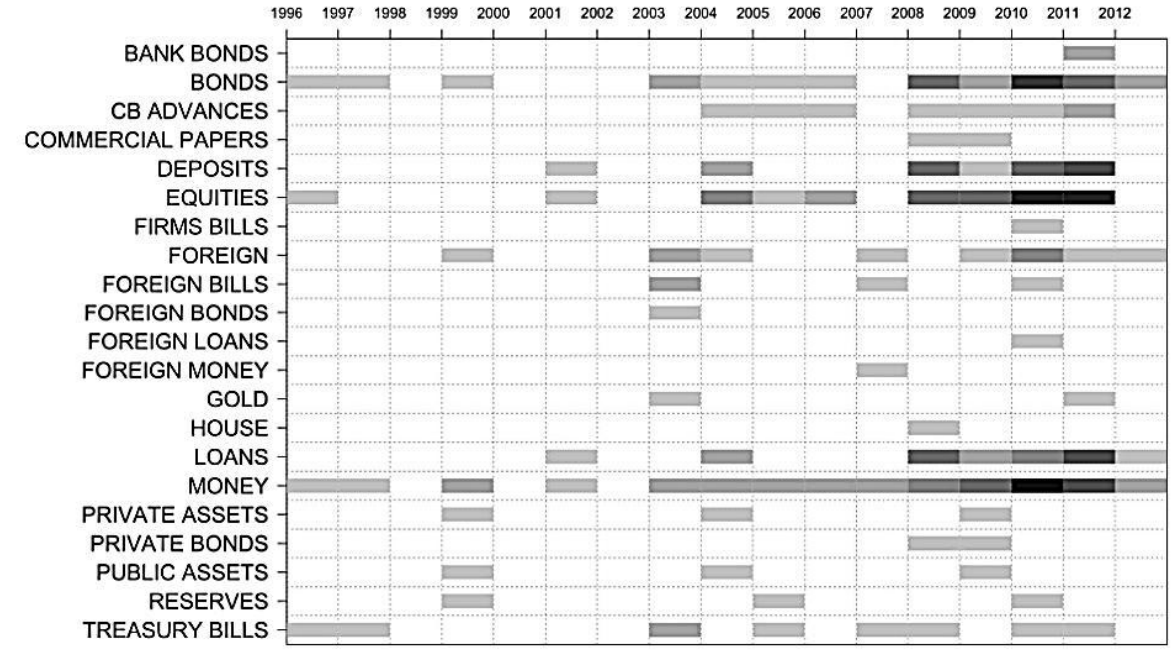
\includegraphics[width = 0.9\textwidth]{./figs/Caverzassi_Heatmap.png}
	\caption*{\textbf{Fonte:} \textcite[p.~4]{caverzasi_stock-flow_2013}}
\end{figure}


Compreendidas tais relações, será desenvolvido um modelo SSM-SFC para dar conta das relações entre lado real e financeiro da economia.
Portanto, esta pesquisa segue o caminho aberto por \textcite{brochier_supermultiplier_2018} ao adicionar um tratamento adequado das relações financeiras no SSM por meio da metodologia SFC estendendo as contribuições de: 
(i) \textcite{jorda_great_2016} ao investigar o processo de ``hipotecarização'' sob um prisma pós-keynesiano a partir de uma análise qualitativa comparativa (QCA); 
%(ii) \textcite{serrano_sraffian_1995} ao incluir o investimento residencial na agenda de pesquisa do supermultiplicador sraffiano; 
(ii) \textcite{teixeira_crescimento_2015} ao avaliar a aplicabilidade da taxa própria de juros dos imóveis para além dos Estados Unidos e;
(iii) \textcite{da_silveira_investimento_2019} ao conectar as relações entre o mercado imobiliário e de crédito diante das especificidades institucionais destacas anteriormente por meio de um modelo SFC de simulação. 




\begin{quote}
	\textit{On the one hand, the German housing
		market was one of the few markets in Western Europe that was not severely affected by the
		global housing boom of the early 2000s. On the other hand, recent developments suggest
		that the role of finance in the German housing system is \textbf{changing}, but not in the same way as
		in other countries}. \cite[p.~969, grifos adicionados]{wijburg_alternative_2017}
\end{quote}

\footnote{Apenas para ilustrar a pluralidade de temas que tal metodologia já abordou, temos --- mesmo que em sua forma mais originária encontrada em \textcite{godley_macroeconomics_1983} --- as formas de financiamento das firmas \cites{asimakopulos_kalecki_1983}{skott_finance_1988}{messori_financing_1991}; endogeneidade da moeda e importância do sistema bancário \cites{messori_financing_1991}{dow_horizontalism:_1996}{arestis_theoretical_1996}{godley_money_1999}; endividamento, distribuição de renda e, apenas para restringir os temas, financeirização \cites{palley_inside_1996}{wolfson_irving_1996}{palley_money_1997}{palley_financial_2002}{dos_santos_revisiting_2009}{palley_inside_2010}{hein_finance-dominated_2012}.}

Sendo assim, o investimento residencial no trabalho de \textcite{nikolaidi_securitisation_2015} possui tanto uma parcela autônoma em relação à renda quanto outra induzida pela renda disponível das famílias.
No entanto, ao partir do procedimento de \textcite{godley_money_1999} para determinação do portfólio de ativos dos agentes, trata os imóveis como um ativo financeiro qualquer sem considerar suas particularidade, qual seja, durabilidade e baixo risco. %TODO: Rever particularidade dos imóveis.


Um  exemplo é o trabalho de  em que são investigados os efeitos da diminuição --- apesar da distribuição da renda a favor dos lucros --- da propensão média a poupar da economia norte-americana por meio da introdução do mercado imobiliário na metodologia SFC\footnote{
	Tal resultado, argumenta, decorre dos ganhos de capital nos mercados imobiliário e acionário entre o topo da distribuição, contribuindo para a diminuição da taxa de poupança.
}. 
Por mais que este trabalho seja uma via para a inclusão do investimento residencial nos modelos macroeconômicos, tal gasto não é o principal determinante da dinâmica  uma vez que parte de uma especificação kaleckiana do investimento das firmas.
Sendo assim, 

Alguns trabalhos seguiram a contribuição de \textcite{zezza_u.s._2008}.
Um deles é o de  com dois tipos de agentes demandando imóveis: parcela dos trabalhadores e investidores institucionais.
Para os primeiros, a demanda por casas é determinada positivamente pela poupança deste setor acrescido de empréstimos hipotecários e negativamente pelo preço dos imóveis de modo que não pode ser considerado estritamente autônomo.
Já os demais agentes, demandam imóveis tal como outros ativos financeiros, ou seja, depende positivamente de sua taxa de retorno.
Em conjunto, tais equações comportamentais determinam que a taxa de crescimento do investimento residencial depende tanto da razão entre a demanda por imóveis em relação ao total quanto de sua inflação que, por sua vez, é determinada pelo estoque de imóveis não vendidos.


%%%%%% ANÁLISE INSTITUCIONAL COMPARATIVA A PARTIR DA NEI -> CHANG: CONFIGURAÇÕES DIFERENTES LEVAM ÀS MESMAS FUNÇÕES. %%%%
A literatura sobre análise institucional comparada se deve, em grande medida, aos desenvolvimentos da Nova Economia Institucional (MENARD e SHIRLEY).
Tal abordagem, no entanto, não faz uma distinção entre formas e funções das instituições além de partir do paradigma ``one-fits-all'' (CHANG 2007, Ch2).
CHANG 2011, por outro lado, argumenta que  diferentes arranjos institucionais podem desempenhar (conjuntamente) as mesmas funções. 
Dito isso, a presente pesquisa parte desta hipótese de ausência de uniformidade causal do arranjo institucional e, assim, enfatizará as particularidades de cada país.



\end{comment}
\section{Objetivos}\label{OBJ}

O \textbf{objetivo geral} da tese é investigar as implicações macroeconômicas do mercado imobiliário e suas relações com as instituições, inflação de ativos e instabilidade financeira. 
% tendo em vista sua relevância macroeconômica. 
Parte-se de uma abordagem multidimensional para contemplar seus principais elementos teóricos e empíricos, visando integrar o lado real ao financeiro dando a devida atenção às instituições. %, são eles: (i) institucionais; (ii) dinâmicos e; (iii) integração do lado real e financeiro.
Cada objetivo específico é o desdobramento de uma dessas dimensões da assim chamada macroeconomia imobiliária cujas metodologias e procedimentos são detalhados na seção seguinte. 

O \textbf{primeiro} objetivo específico consiste em examinar as configurações institucionais que determinam o grau de hipotecarização do sistema bancário de um país a partir de uma análise qualitativa comparada (do inglês, QCA). A partir deste modelo, é possível encontrar as condições necessárias e suficientes para explicar o porquê de alguns sistemas bancários possuírem uma maior participação relativa das hipotecas nos balanços das instituições financeiras.
%A importância desta contribuição também se dá pela possibilidade de extrapolar o potencial explicativo de tais configurações institucionais para além dos países presentes na base de dados de \textcite{jorda_rate_2019} e inferir os respectivos graus de hipotecarização.

O \textbf{segundo} objetivo específico é explorar alguns fatos estilizados da macroeconomia imobiliária e, em particular,  estimar os determinantes do investimento residencial tendo em vista sua relevância para a dinâmica macroeconômica. 
A importância deste modelo é uma melhor compreensão da relação entre investimento residencial, concessão de crédito e bolha de ativos. %a possibilidade de se investigar as implicações do investimento residencial para o endividamento das famílias; preço dos imóveis; crescimento econômico e estabilidade financeira.
Para tanto, desenvolve-se um modelo de séries temporais em painel para os países presentes na base de dados de \textcite{jorda_rate_2019}. 

Por fim, o \textbf{terceiro} objetivo específico é avaliar as implicações macroeconômicas de um sistema bancário ativo com racionamento de crédito por meio de um modelo AB-SFC de simulação com famílias heterogêneas e investimento residencial explicitamente modelado. 
Desse modo, ao integrar o lado real e financeiro da macroeconomia imobiliária é possível desenvolver um modelo teórico no qual o financiamento dos imóveis desempenha um papel central.
Este modelo permitirá análises mais elaboradas dos efeitos das bolhas de ativos na demanda agregada; taxa de crescimento econômico; endividamento das famílias (heterogêneas); composição patrimonial dos bancos e; estabilidade financeira.
%Além disso,  uma melhor compreensão da heterogeneidade das famílias para a dinâmica dos fluxos e dos estoques permite investigar a ``Nova Narrativa''. 


\begin{comment}
\begin{description}
	\item[Objetivo geral] Investigar as implicações macroeconômicas dos imóveis.
	\item[Objetivos específicos] {\color{white}Teste}
	\begin{itemize}
		\item Examinar as configurações institucionais da ``hipotecarização'';
		\item Estimar os principais determinantes macroeconômicos do investimento residencial;
		\item Avaliar as implicações de um sistema bancário ativo e de bolha de ativos com ciclo de crédito endógeno por meio de um modelo AB-SFC com famílias heterogêneas e investimento residencial autônomo.
	\end{itemize}
\end{description}
\end{comment}

\section{Metodologia}\label{passos}
%TODO: Marcar. Me atentei para deixar essa seção sempre no futuro.

Para atender os objetivos, a pesquisa será dividida em três capítulos independentes.
O primeiro tratará das especificidades institucionais da aqui denominada macroeconomia imobiliária por meio de uma análise qualitativa comparativa.
No capítulo seguinte, será estimado um modelo de séries temporais em painel para analisar os determinantes do investimento residencial.
Em seguida, será elaborado um modelo AB-SFC com famílias heterogêneas para avaliar as implicações de bolha de ativos e racionamento de crédito.


\subsection{Especificidades institucionais da macroeconomia imobiliária}

Nos últimos anos, nota-se um aumento dos estudos que destacam o potencial explicativo das instituições em uma perspectiva comparada com especial ênfase no setor financeiro\footnote{
    \textcite{blackwell_origins_2018}, por exemplo, discutem as origens da institucionalidade bancária e financeira do mercado de hipotecas. \textcite{van_gunten_varieties_2018}, por sua vez, analisam mudanças institucionais na oferta de crédito em Portugal, Espanha, França e Alemanha e concluem que tais mudanças foram responsáveis pela maior intensificação financeira das famílias.
}.
Dentro deste paradigma, a literatura de Economia Política Comparada (CPE, no inglês) se destaca por conceituar o papel macroeconômico deste setor institucional.
No entanto, a vertente predominante da CPE (``Variedade de Capitalismos'', em inglês, VoC) tem redirecionado atenção a questões microeconômicas e relacionadas à oferta de crédito \cite{schwartz_thinking_2019}.
Recentemente, há um esforço de conectar tal abordagem comparativa aos modelos de crescimento liderados pela demanda em que o endividamento das famílias  é central \cite{baccaro_rethinking_2016}.
No entanto, 
estes modelos %\textcite{baccaro_rethinking_2016} 
não dão a devida atenção à composição e aos determinantes do crescimento do setor financeiro que, como visto, não podem ser desassociados do mercado imobiliário e das hipotecas \cite{wood_house_2020}.

Uma literatura que dá muita atenção aos fenômenos associados à aqui denominada macroeconomia imobiliária é a da financeirização que analisa, principalmente, as relações entre investimento produtivo, instabilidade financeira e crescimento \cites{stockhammer_financialisation_2004}{hein_demise_2015}{detzer_financialization_2019}. %\cites{stockhammer_financialisation_2004}{orhangazi_financialisation_2008}{hein_demise_2015}{detzer_financialization_2019}.
Além de não dar atenção às famílias e ao investimento residencial --- limitando-os à subprocessos da financeirização \cites{aalbers_financialization_2008}{schwartz_politics_2009}{bibow_financialization_2010} ---, esta literatura pouco tem avançado em uma análise institucional comparada. 
Todos os trabalhos que o fazem se restringem a um número pequeno de países nas suas amostras \cites{becker_peripheral_2010}{lapavitsas_financialisation_2013}. % em que analisam apenas quatro economias em ambos os trabalhos. %%% KARWARZASKI ANALISA VÁRIOS, MAS USA CORRELAÇÃO E NÃO É POSSÍVEL AVALIAR CONDIÇÕES NECESSÁRIAS E SUFICIENTES

Uma exceção é o trabalho de \textcite{karwowski_financialisation_2019} que avalia as diferentes consequências da financeirização para as famílias, firmas e bancos em 17 países da OCDE por meio do coeficiente de correlação de postos de Spearman, concluindo que o preço dos ativos (sobretudo imóveis) são relevantes para explicar o endividamento das famílias.
No entanto, este estudo não permite avaliar quais configurações institucionais são necessárias ou suficientes para explicar como a inflação de ativos está conectada com esse aumento dos passivos das famílias.
\textcite{mertzanis_financialisation_2019}, por sua vez, investiga os determinantes do acesso ao crédito para as firmas em 138 economias em desenvolvimento por meio de modelo \textit{probit} com \textit{dummies} institucionais e conclui que tais variáveis não só determinam o acesso ao financiamento como também amenizam as restrições financeiras das firmas.
Entretanto,  tal análise só permite investigar os efeitos marginais das instituições.
Sendo assim, conclui-se que estas análises comparativas para médias e grandes amostras carecem de um aparato metodológico mais adequado para tratar das instituições qualitativamente.


Desta discussão, conclui-se que os autores da financeirização, CPE e VoC que partem de uma perspectiva institucional comparada dão maior ênfase ao desempenho das firmas enquanto uma parcela menor analisa as famílias.
O aumento sem precedentes das hipotecas no balanço patrimonial dos bancos reportado por \textcite{jorda_great_2016} evidencia  que a pouca atenção dada às famílias, ao investimento residencial e às hipotecas é desproporcional à relevância que tais elementos possuem na dinâmica financeira recente. 
No entanto, mesmo os trabalhos que tocam os temas da aqui denominada macroeconomia imobiliária dão pouca ênfase às institucionalidades do mercado imobiliário em particular.
Por exemplo, \textcite{wijburg_alternative_2017} destacam que a especificidade institucional do mercado imobiliário alemão o configura como um contraponto ao norte-americano pela baixa liquidez do mercado hipotecário e que tal particularidade condiciona a relação entre preço dos imóveis, investimento residencial e crescimento econômico. %%%% EXEMPLOS
\textcite{johnston_global_2017}, por sua vez, reportam a importância das instituições na determinação dos preços dos imóveis enquanto \textcite{fuller_housing_2020} encontram evidências que a trajetória deste preço é relevante para explicar a concentração da riqueza em alguns países europeus.

Além de não tratar dos temas da macroeconomia imobiliária conjuntamente, a literatura não tem investigado o porquê de alguns sistemas bancários apresentarem um maior grau de hipotecarização que outros e esta é uma das lacunas a ser preenchida por esta tese.
%Ao longo desta pesquisa, 
Argumenta-se que a regularidade encontrada por \textcite{jorda_great_2016}
não significa que a especificidade de cada país deixa de ser relevante. 
%e, assim, parte das instituições formais de cada pais para avaliar 
Seguindo \textcite{chang_institutions_2011},  parte-se da hipótese de ausência de uniformidade causal do arranjo institucional.
Apropriando esta fundamentação teórica ao objeto desta tese,  assume-se que diferentes configurações institucionais podem desempenhar as mesmas funções e explicar o grau de hipotecarização. %dos sistemas bancários.

A tabela \ref{Institucional} reúne algumas características institucionais tratadas dispersamente pela literatura que dizem respeito às relações entre famílias, bancos e mercado imobiliário para alguns dos países presentes na base construída por \textcite{jorda_rate_2019}. São elas: 
    (i) maturidade das hipotecas \cite{green_american_2005}; 
    (ii) determinação  e tipo da taxa de juros das hipotecas (fixa ou flexível); 
    (iii) arranjo regulatório sobre quitação antecipada do crédito imobiliário (contrato ou legislação) e formas de refinanciamento;
    (iv) possibilidade de uma segunda hipoteca a partir da valorização do imóvel;
    (v) disponibilidade de crédito de longo-prazo para as famílias \cite{schwartz_politics_2009} e; 
    (vi) possibilidade de transferência de riscos (\textit{e.g.} securitização \cite{european_central_bank_housing_2010}).
    
    



\begin{table}[htb]
	\centering
	\caption{Características institucionais de alguns países europeus da OCDE}
	\label{Institucional}
		\resizebox{.7\textwidth}{!}{%
			\begin{tabular}{c|c|c|c|c|c|c}
				\hline\hline \\
				\multirow{2}{*}{\textbf{Países}} & \multicolumn{6}{c}{\textbf{Características institucionais}} \\\cline{2-7}
				&
				\textbf{\begin{tabular}[c]{@{}c@{}}Maturidade\\ Hipotecária\\(meses)\end{tabular}} &
				\textbf{\begin{tabular}[c]{@{}c@{}}Taxa de juros\\ Hipotecária\end{tabular}} &
				\textbf{\begin{tabular}[c]{@{}c@{}}Reembolso antecipado:\\ Contratado (C)/\\ Legislado (L)\end{tabular}} &
				\textbf{\begin{tabular}[c]{@{}c@{}}Possibilidade de segunda\\hipoteca a partir\\da valorização do imóvel\end{tabular}} &
				\textbf{\begin{tabular}[c]{@{}c@{}}Financiamento pelo\\ Mercado de capitais (\%)\end{tabular}} &
				\textbf{\begin{tabular}[c]{@{}c@{}}Execução\\ Hipotecária\\(meses)\end{tabular}} \\\hline
				\textbf{Alemanha}                & 30   & Fixa       & C/L   & Não permitido    & 14   & 9    \\\hline
				\textbf{Espanha}                 & 30   & Variável   & C/L   & Limitado         & 45   & 8    \\\hline
				\textbf{França}                  & 19   & Fixa       & C/L   & Não permitido    & 12   & 20   \\\hline
				\textbf{Holanda}                 & 30   & Fixa       & C     & Permitido        & 25   & 5    \\\hline
				\textbf{Itália}                  & 22   & Variável   & L     & Não permitido    & 20   & 56   \\\hline
				\textbf{Portugal}                & 40   & Variável   & L     & Sem informação   & 27   & 24  \\\hline
				\hline
				
			\end{tabular}%
		}
	\caption*{\textbf{Fonte:}  \textcite[p.~94, adaptado e traduzido]{van_gunten_varieties_2018}}
\end{table}
Uma breve inspeção da tabela \ref{Institucional} revela uma pluralidade de configurações institucionais no que dizem respeito ao mercado de crédito imobiliário. 
Apesar desta pluralidade institucional, destaca-se que a hipotecarização é um fenômeno comum a estes países.
Sendo assim, pontua-se a necessidade de se investigar quais desses arranjos institucionais propiciam um maior ou menor grau de hipotecarização.
Diferentemente de \textcites{karwowski_financialisation_2019}{mertzanis_financialisation_2019}, a presente pesquisa propõe uma análise institucional centrada em variáveis qualitativas e se difere da proposta de \textcites{becker_peripheral_2010}{lapavitsas_financialisation_2013} ao analisar um número maior de casos sem que, para isso, abandone a relevância das particularidades de cada país.
Sendo assim, ao partir de um aparato metodológico mais adequado para tratar de variáveis qualitativas, é possível investigar diferentes configurações institucionais e compreender em que medida estes elementos ajudam a compreender os determinantes necessários e suficientes da hipotecarização.

\begin{comment}
Por mais que estes trabalhos lancem luz sobre as implicações das instituições sobre a financeirização, não é possível 

tais análises só permite investigar os efeitos marginais uma vez que parte de uma especificação econométrica.

Como visto, \textcite{jorda_great_2016} reportam um aumento sem precedentes da participação das hipotecas no balanço patrimonial dos bancos. 


No entanto, ao partir de correlações, o estudo de \textcite{karwowski_financialisation_2019} não permite avaliar quais configurações são necessária ou suficientes para explicar o aumento das diferentes dimensões da financeirização.
No que diz respeito especificamente às configurações institucionais, o autor conclui que tais variáveis determinam o acesso ao financiamento e atenuam o impacto da financeirização.

Sendo assim, a pouca atenção dada às famílias, ao investimento residencial e às hipotecas é desproporcional à relevância que tais elementos possuem na dinâmica financeira recente.
\end{comment}


\subsection{Implicações do investimento residencial para a dinâmica macroeconômica}

No pós-Grande Recessão, nota-se um maior interesse nas implicações macroeconômicas do investimento residencial   \cites{leamer_housing_2015}{teixeira_crescimento_2015}{fiebiger_trend_2017}.
Apesar da existência de alguns trabalhos empíricos evidenciando este gasto como um indicador antecedente para reversões do ciclo econômico no período do pós-guerra \cites{green_follow_1997}{leamer_housing_2007}, a atenção ao tema foi esparsa e assistemática.
%Dentre as exceções, 
\textcite{duesenberry_investment_1958} foi um dos poucos a reportar a importância do investimento residencial e da inflação de imóveis para explicar o ciclo econômico muito antes da Grande Recessão. 
Outro exemplo é o de \textcite{keynes_collected_1978} que em carta ao Presidente dos EUA Franklin D. Roosevelt escreveu sobre a relevância dos imóveis para a recuperação econômica no contexto da Grande Depressão: % conforme o trecho da carta transcrito abaixo:

\begin{quote}
    `` [...] \textit{Housing is by far the best aid to recovery because of the large and continuing scale of potential demand; because of the wide geographical distribution of this demand; and because the sources of its finance are largely independent of the stock exchanges. I should advise putting most of your eggs in this basket, caring about this more than about anything, and making absolutely sure that they are being hatched without delay. In this country we partly depended for many years on direct subsidies. 
    There are few more proper objects for such than working-class houses.% If a direct subsidy is required to get a move on (we gave our subsidies through the local authorities), it should be given without delay or hesitation
    }''
    \cite[p.~436]{keynes_collected_1978}
\end{quote}

Nos últimos anos, a literatura econométrica tem evidenciado que a relevância do investimento residencial não se restringe à Grande Recessão nem aos EUA. 
Enquanto alguns trabalhos reportam que tal investimento antecede o ciclo econômico para um conjunto considerável de países \cites{gauger_residential_2003}{huang_is_2018}, outros enfatizam o efeito riqueza (via valorização dos imóveis) sobre o consumo das famílias em diversas economias desenvolvidas \cite{de_bandt_housing_2010}. %{arrondel_housing_2010}. 
Mais recentemente, alguns autores têm evidenciado a relevância da inflação de imóveis na determinação do endividamento das famílias, da distribuição de riqueza e da estabilidade macroeconômica 
%\cites{hofmann_determinants_2004}{goodhart_house_2008}{dieci_simple_2009}{ryoo_household_2015}{stockhammer_debt-driven_2016}{barnes_private_2016}{johnston_global_2017}{mian_household_2017}{anderson_politics_2020}{fuller_housing_2020}.
\cites{ryoo_household_2016}{stockhammer_debt-driven_2016}{barnes_private_2016}{johnston_global_2017}{mian_household_2017}{anderson_politics_2020}{fuller_housing_2020}.
%Portanto, as implicações do investimento residencial para a dinâmica macroeconômica apontadas pela literatura vão além de seus impactos sobre o crescimento.

Apesar de dispersa, nota-se que a literatura econométrica sobre as implicações macroeconômicas do investimento residencial é crescente.
%Sendo assim, dada a relevância deste gasto para a dinâmica macroeconômica, se faz necessário compreender seus determinantes.
No entanto,     a partir da revisão de literatura, nota-se que os modelos econométricos %estão mais centrados nas consequências e menos nos seus determinantes de modo que 
pouco avançaram no tratamento teórico dos determinantes do investimento residencial. 
Um exemplo desta lacuna é o trabalho de \textcite{wood_house_2020} em que os autores avaliam a relação entre crescimento, endividamento das famílias e preço dos imóveis.
Para tanto, estimam um modelo autorregressivo de defasagem distribuída (no inglês, ARDL)  para 18 economias avançadas para os anos de 1980 a 2017 e concluem que o preço dos imóveis determina o endividamento das famílias que, por sua vez, é fundamental para explicar o crescimento recente dos países analisados.
Por mais que o trabalho de \textcite{wood_house_2020} evidencie a relevância do preço dos imóveis e do crédito imobiliário para a dinâmica macroeconômica, o faz sem considerar o investimento residencial e seus determinantes. 
Uma exceção é o estudo de 
%\textcite{poterba_tax_1984} cuja especificação do investimento residencial depende positivamente do preço dos imóveis. Por mais que este trabalho seja pioneiro ao não pressupor que a oferta de imóveis tende instantaneamente ao nível desejado, não inclui bolha de ativos. 
%Diante desta omissão, 
\textcite{arestis_residential_2015} que estima os determinantes do investimento residencial por meio de um modelo ARDL para 17 países da OCDE.  
Dentre as conclusões, destaca-se que o preço dos imóveis e o acesso ao crédito são os principais determinantes deste gasto.

Uma alternativa para se estimar o investimento residencial é por meio da taxa própria de juros dos imóveis. 
Desenvolvido por \textcite{teixeira_crescimento_2015}, este conceito é definido pelo deflacionamento da taxa de juros das hipotecas pela inflação de imóveis e foi elaborado para examinar a bolha imobiliária ocorrida nos EUA nos anos 2000.
Diferentemente de um deflacionamento por um índice geral de preços, como faz \textcite{fair_macroeconometric_2013}, este constructo teórico permite  auferir o custo real em imóveis de se comprar imóveis \cite[p.~53]{teixeira_crescimento_2015}\footnote{Destaca-se também que em momentos de bolha de imóveis é a inflação destes ativos que domina a dinâmica da taxa própria \cite[p.~53]{teixeira_crescimento_2015}. Sendo assim, quanto menor esta taxa, maiores serão os ganhos de capital (em imóveis) por se especular com imóveis.}. 
Portanto, trata-se da taxa de juros relevante para os demandantes de casas.
%Partindo desta taxa de juros real específica, 
\textcite{petrini_demanda_2019} estimou um modelo econométrico para os EUA entre os anos de 1992 a 2019 e encontra evidências empíricas que a taxa própria de juros dos imóveis é uma variável relevante para explicar a taxa de crescimento do investimento residencial e que estas variáveis são cointegradas.
Desta revisão de literatura, destaca-se que  os poucos trabalhos que analisam os determinantes do investimento residencial têm examinado os EUA em específico como é o caso de \textcite{teixeira_crescimento_2015} e de \textcite{petrini_demanda_2019}. 
%Em especial, destaca-se que apesar de alguns trabalhos evidenciarem a relevância do investimento residencial para a dinâmica macroeconômica, o fazem sem considerar sem investigar seus determinantes.
%Além disso, parte expressiva desta literatura tem examinado os EUA em específico como é o caso de \textcite{teixeira_crescimento_2015} por meio da taxa própria de juros dos imóveis.

Dessa discussão, pontuou-se a necessidade de se estudar a dimensão quantitativa da macroeconomia imobiliária. % se dá pela importância do investimento residencial sobre a dinâmica de crescimento; pela relevância da inflação dos imóveis sobre o endividamento das famílias e distribuição pessoal da riqueza e; pelo crescimento do crédito e do setor financeiro ter sido liderado principalmente pelas hipotecas  (hipotecarização).
%Portanto, esta pesquisa é um esforço de reunir tais elementos que, como visto, estão dispersos na literatura.
Em particular, dada a importância do investimento residencial para a dinâmica macroeconômica, esta pesquisa propõe explorar os fatos estilizados que dizem respeito ao investimento residencial e 
investigar seus determinantes por meio de um modelo econométrico.
%Esta pesquisa propõe investigar  a aplicabilidade deste constructo teórico para outros países uma vez que \textcite{petrini_demanda_2019} encontrou uma elevada capacidade explicativa desta variável para os EUA.
Sendo assim, esta investigação se difere de \textcite{wood_house_2020} ao investigar os determinantes do investimento residencial; de \textcite{arestis_residential_2015} ao enfatizar a relevância da bolha de ativos por meio de uma taxa de juros real específica e; conforme será discutido na seção \ref{metodologia2}, de \textcite{teixeira_crescimento_2015} e de \textcite{petrini_demanda_2019} ao ampliar o escopo de análise para mais países. 









%Apesar desta taxa própria explicar a dinâmica da taxa de crescimento do investimento residencial econometricamente,  e, portanto, não foi feita uma investigação a respeito da aplicabilidade para outros países e este é um dos objetivos desta pesquisa.

%%%%%%%%%%%%%%%%%%%%%%%%%%%%% Escrever o que será feito %%%%%%%%%%%%%%%%%%

\begin{comment}
\textcite{alvarez_does_2010}, por exemplo, concluem que tal tipo de investimento antecede o ciclo econômico para o caso espanhol e resultados semelhantes podem ser encontrados para França, Espanha  e Itália enquanto o caso alemão apresenta uma dinâmica distinta \cite{de_bandt_housing_2010}. 
Outros estudos empíricos, por sua vez, têm enfatizado o efeito riqueza --- via valorização dos imóveis --- sobre o consumo e indicam tais canais de transmissão são mais incidentes, em ordem, sobre Estados Unidos e Grã Bretanha e mais brandos no caso francês e alemão \cites{de_bandt_housing_2010}{arrondel_housing_2010}.

Tal como pontuado por \textcite{jorda_great_2016}, o crescimento do crédito e do setor financeiro tem sido liderado principalmente pelas hipotecas.
Como consequência, as atividades bancárias se reorientaram para a concessão de crédito às famílias e não para o investimento produtivo \cites{erturk_banks_2007}{kohl_more_2018}.
%Sendo assim, para dar conta das implicações dinâmicas da macroeconomia imobiliária, é preciso considerar outros elementos.
%Em outras palavras, a literatura empírica tem apontado para uma tendência comum entre um conjunto de variáveis que precisa ser melhor analisada.
%%%%%%%%%%%%% Uma parcela menor de trabalhos associam os movimentos do mercado imobiliario com as condições de financiamento das firmas.
Em paralelo, pontua-se um crescente consenso da literatura sobre a relevância dos elementos que constituem a aqui determinada macroeconomia imobiliária.

\footnote{
    A razão disso é que os imóveis são  uma das formas de riqueza mais comuns entre as famílias norte-americanas e serviam --- principalmente nos anos 2000 --- de colateral para tomada de crédito \cites{teixeira_uma_2011}{hay_failure_2013}. A forma de ``realizar'' o ganho de capital com a bolha imobiliária que ocorreu no período, sem precisar liquidá-los, era justamente ampliando o endividamento à medida que este colateral aumentava de valor \cite{teixeira_crescimento_2015}. 
}. 


Embora a relevância do investimento residencial para a dinâmica macroeconômica não se restrinja aos EUA, parte expressiva desta literatura tem examinado este caso em específico\footnote{
    A razão disso é que os imóveis são  uma das formas de riqueza mais comuns entre as famílias norte-americanas e serviam --- principalmente nos anos 2000 --- de colateral para tomada de crédito \cites{teixeira_uma_2011}{hay_failure_2013}. A forma de ``realizar'' o ganho de capital com a bolha imobiliária que ocorreu no período, sem precisar liquidá-los, era justamente ampliando o endividamento à medida que este colateral aumentava de valor \cite{teixeira_crescimento_2015}. 
}. 



Por mais que alguns trabalhos têm evidenciado a relevância do investimento residencial para a dinâmica macroeconômica, o fazem sem considerar sem investigar seus determinantes.
Além disso, parte expressiva desta literatura tem examinado os EUA em específico como é o de\footnote{
    A razão disso é que os imóveis são  uma das formas de riqueza mais comuns entre as famílias norte-americanas e serviam --- principalmente nos anos 2000 --- de colateral para tomada de crédito \cites{teixeira_uma_2011}{hay_failure_2013}. A forma de ``realizar'' o ganho de capital com a bolha imobiliária que ocorreu no período, sem precisar liquidá-los, era justamente ampliando o endividamento à medida que este colateral aumentava de valor \cite{teixeira_crescimento_2015}. 
}. 
\end{comment}

\subsection{Dimensão real e financeira do mercado imobiliário}

%%%%%%%%%%%%%%%%%%%%%%%%%%%%%%%%% APRESENTAÇÃO DO PROBLEMA %%%%%%%%%%%%%%%%%%%%%%%%%%
% Apresentação da velha narrativa %
Há um relativo consenso na literatura \textit{mainstream} de que a concessão de crédito às famílias com pior avaliação de risco está na origem da Grande Recessão\footnote{
Um exemplo deste consenso é o livro de \textcite{mian_consequences_2009}.
}. 
% Apresentação do geral: Jordà %
%Partindo de uma base de dados inédita, \textcite{jorda_great_2016} reportam que o crédito concedido às famílias cresceu a uma taxa maior do que para os demais setores não-financeiros de modo que  a intermediação financeira tem alterado o \textit{locus} do risco para os empréstimos imobiliários e hipotecas e que esta dinâmica contribui para a ocorrência de crises financeiras \cite{schularick_credit_2012}.
% Apresentação do específico: nova narrativa %
No entanto, evidências recentes sugerem uma ``nova narrativa'' \cite{albanesi_credit_2017}: os agentes melhor avaliados pelos bancos foram aqueles que adquiriram imóveis para fins especulativos/diversificação de portfólio e apresentaram maiores taxas de \textit{default}; enquanto a concessão de crédito e a taxa de \textit{default} entre aqueles com pior avaliação de risco se mantiveram constantes ao longo da bolha imobiliária.
% TODO Marcar daqui até o fim. Fala que tem um backup da versão anterior. 
Este resultado decorre, em um primeiro momento, da valorização dos imóveis como colateral seguido do esgotamento da bolha imobiliária (pós-2005).
A subsequente desvalorização destes ativos não foi acompanhada pela redução dos compromissos financeiros das famílias (dívida). 
% Backup: Este resultado está associado tanto à valorização dos imóveis como colateral quanto ao descolamento entre os ativos e passivos  das famílias ao longo da crise. Este descolamento decorre tanto do esgotamento da bolha dos imóveis (pós-2005) que fez com que os tais ativos desvalorizassem quanto da insensibilidade dos compromissos financeiros das famílias (dívida) a queda do preço de seus ativos.
Em outras palavras, os imóveis (ativo) têm valor de mercado enquanto a dívida (passivo) tem um valor contratual de modo que o patrimônio líquido das famílias cai  enquanto sua fragilidade financeira aumenta com o instaurar da crise \cites{albanesi_credit_2017}{jorda_rate_2019}.
%O movimento subsequente é caracterizado pelo que \textcite{koo_holy_2009} denominou de ``recessão de balanço patrimonial'' (no original, \textit{balance sheet recession})  em que parte considerável da poupança das famílias é destinada ao pagamento de amortização da dívida para se desalavancar e isso tem implicações negativas para a retomada\footnote{Originalmente, este conceito foi desenvolvido no contexto do estouro da bolha imobiliária no Japão nos anos 1990 e recentemente tem sido utilizado para explicar o pós-Grande Recessão.}.


%%%%%%%%%%%%%%%%%%%%%%%%%%%%%%%%%%%%%%%%% RELEVANCIA DO SFC %%%%%%%%%%%%%%%%%%%%%%%
Dentre os poucos economistas que anteciparam a Grande Recessão, \textcite{godley_seven_1999} se destaca pela sua contribuição metodológica: a abordagem consistente entre fluxos e estoques (adiante, SFC)\footnote{Cabe ressaltar que apesar da metodologia SFC ter recebido uma maior atenção no pós Grande Recessão, é uma proposta de análise cujas origens datam desde os anos 70. Sobre as origens desta metodologia, suas hipóteses explícitas e implícitas, ver \textcite{teixeira_crescimento_2015}.}.
Nos últimos anos, houve um crescente consenso na literatura heterodoxa de que esta metodologia é uma das melhores formas de modelar a conexão do lado real ao financeiro da economia \cite{nikiforos_stock-flow_2017}.
% Lacuna 1: poucos olham investimento residencial %
Apesar da crescente aceitação desta metodologia pela literatura, os imóveis estão entre os ativos menos analisados  \cite{caverzasi_stock-flow_2013}.
%% Petrini e Teixeira %
Uma exceção é o modelo de \textcites{petrini_demanda_2019}{petrini_long_2020} em que são incluídos crédito às famílias e firmas; investimento residencial e bolha de ativos.
Diferente de \textcite{zezza_u.s._2008} e \textcite{nikolaidi_securitisation_2015}, os autores partem do supermultiplicador sraffiano de modo que é o investimento residencial que lidera o ciclo econômico\footnote{
    Desenvolvido originalmente por \textcite{serrano_sraffian_1995}, o supermultiplicador sraffiano tem sido utilizado por um conjunto de autores mais amplo como é o caso de \textcites{allain_tackling_2015}{lavoie_convergence_2016}{serrano_sraffian_2017}{dutt_observations_2018} e, mais recentemente, sido incluído na estrutura contábil SFC por \textcites{brochier_supermultiplier_2018}{mandarino_workers_2020}.
}.
Sendo assim,  tal modelo enfatiza as implicações das bolhas de ativos (neste caso, imóveis) sobre o crescimento econômico e acumulação de capital.
Apesar de analisar as implicações macroeconômicas do investimento residencial, o modelo de \textcite{petrini_demanda_2019} carece de uma melhor representação da relação entre o mercado imobiliário e de crédito, bem como composição patrimonial dos bancos e esta é uma das lacunas a ser preenchida por esta pesquisa.


%Partindo de uma base de dados inédita, \textcite{jorda_great_2016} reportam que o crédito concedido às famílias cresceu a uma taxa maior do que para os demais setores não-financeiros de modo que  a intermediação financeira tem alterado o \textit{locus} do risco para os empréstimos imobiliários e hipotecas e que esta dinâmica contribui para a ocorrência de crises financeiras \cite{schularick_credit_2012}.
%Desse modo, 
Para dar conta das implicações reais e financeiras da macroeconomia imobiliária, se faz necessário compreender as relações entre a composição patrimonial dos bancos e a fragilidade financeira das famílias.
Uma literatura que dá atenção a alguns desses temas é a que parte das contribuições de Hyman Minsky.
Na literatura, somente o trabalho de \textcite{ryoo_household_2016} relaciona o endividamento e a fragilidade financeira das famílias às bolhas de ativos \cite{nikolaidi_minsky_2017}. 
%Ao avaliar esta famílias de modelos que seguem a metodologia SFC, \textcite{nikolaidi_minsky_2017} identificam somente o trabalho de \textcite{ryoo_household_2016} analisa o endividamento e a fragilidade financeiras das famílias conjuntamente. 
Neste modelo, são os trabalhadores --- e não os rentistas --- que investem em imóveis e o fazem a partir da taxa de retorno esperada ao se especular com casas\footnote{Cabe destacar que o trabalho de \textcite{ryoo_household_2016} se baseia em normas estoque-fluxo exogenamente determinadas de modo que ciclos financeiros no modelo também se tornam exógenos.}.
Apesar de avançar em direção a um maior esclarecimento na relação entre bolha de ativos e instabilidade financeira das famílias, as hipóteses do modelo de \textcite{ryoo_household_2016} podem ser questionadas uma vez que \textcite{albanesi_credit_2017} encontraram evidências empíricas de que foram os rentistas ---  e não os trabalhadores --- que especularam com imóveis.
%TODO: Marcar
%%%%%%%%%%%%%%%%%%%%%%%%%%%%%%%%%%%%%%%%% LACUNA SFC %%%%%%%%%%%%%%%%%%%%%%%%%%%%%%%


A partir da revisão de literatura dos modelos SFC, nota-se o pouco detalhamento das relações financeiras entre famílias e bancos \cite{lavoie_was_2020}. %TODO Marcar. Obtei tirar as firmas dessa frase tb. Achei que tirava mto o foco.
Outra lacuna identificada na literatura que parte desta metodologia é o tratamento teórico do setor financeiro em que atua como intermediador bancário \cite{le_heron_post-keynesian_2008}\footnote{\textcite{nikolaidi_minsky_2017} também destacam que a maioria dos modelos minskyanos que partem da metodologia SFC enfatiza o endividamento das firmas e o fazem sem incluir racionamento de crédito.}.
Portanto, os modelos SFC têm dado pouca atenção à relação entre fragilidade financeira das famílias, investimento residencial, racionamento de crédito e bolha de ativos. 
%%%%%%%%%%%%%%%%%%%%%%%%%%%%%%%%%%%%%%%%% LACUNA SFC E COMPLEMENTARIEDADE ABM %%%%%%%%%%%%%%%%%%%%%%%%%%%


Seguindo \textcite{bellofiore_minskys_2001}, destaca-se que a melhor forma de analisar fenômenos como a instabilidade financeira minskyana é por meio de modelos que possuem agentes com comportamentos heterogêneos como é o caso da modelagem baseada em agentes (adiante, ABM).
%%%%%%%%%%%%%%%%%%%%%%%%%%%%%%%%%%%%%%%% LACUNA ABM NÂO SFC%%%%%%%%%%%%%%%%%%%%%%%%%%%%%%%%
%%%%%%%%%%%%%%%%%%%%%%%%%%%%% AB-SFC COM CICLO ENDÓGENO %%%%%%%%%%%%%%%%%%%%%%%%
Uma forma de incluir racionamento de crédito nesta metodologia é a de \textcite{dawid_bubbles_2015} em que os autores analisam as relações entre regulação bancária e ciclo econômico.
No entanto, tal como é usual nesta literatura, racionamento de crédito é exclusivo à relação entre firmas e bancos, enquanto as famílias apenas acumulam riqueza sob a forma de depósitos bancários.
Outros autores que utilizam modelos do tipo ABM têm avaliado as relações entre instabilidade financeira, endividamento das famílias e distribuição de renda.
\textcite{cardaci_inequality_2018} parte da hipótese de consumo cascata para investigar as associações entre a concentração da renda e inflação de imóveis\footnote{
    Em linhas gerais, a hipótese de consumo cascata desenvolvida por \textcite{duesenberry_income_1949} descreve que o aumento do consumo dos percentis mais elevados de renda induzem o aumento do consumo dos percentis inferiores e este efeito é maior quanto maiores forem as disparidades de renda. %\textcite{veblen_theory_1899}
}.
Apesar de relevante, tal contribuição não avança em direção a uma especificação dos determinantes da taxa de crescimento do investimento residencial.
Além disso, tanto \textcite{dawid_bubbles_2015} quanto \textcite{cardaci_inequality_2018} não mapeiam explicitamente as relações entre fluxos e estoques como propõe a metodologia SFC.


%%%%%%%%%%%%%%%%%%%%%%%%%%%%%%%%%%%%%%% RELEVÂNCIA AB-SFC %%%%%%%%%%%%%%%%%%%%%%%%%%
Uma alternativa é o modelo de \textcite{caiani_agent_2016} em que os autores propõem um ABM na estrutura contábil SFC (adiante, AB-SFC) de modo a desfrutar das vantagens de ambas metodologias: emergência de fenômenos macroeconômicos em que estão explicitados todos os \textit{feedbacks} intersetoriais entre fluxos e estoques.
Por mais que o modelo de \textcite{caiani_agent_2016} seja bastante desagregado e detalhado, não inclui tanto bolha de ativos e investimento residencial quanto relações de crédito entre famílias e bancos.
%%%%%%%%%%%%%%%%%%%%%%%%%%%%% AB-SFC PARCIAL, SEM IMÓVEIS %%%%%%%%%%%%%%%%%%%%%%
Uma forma de explicitar as relações entre fluxos e estoques e incluir heterogeneidade dos agentes sem precisar incorrer em um elevado grau de desagregação é por meio de um modelo AB-SFC parcial em que somente alguns agentes possuem comportamento heterogêneo.
Além de ser mais parcimonioso, tal procedimento permite evidenciar a emergência de interações complexas entre os agentes sem que, para isso, seja necessário abrir mão da compreensibilidade do modelo.
Um exemplo desta estratégia é o modelo de \textcite{botta_when_2019} em que os autores investigam as implicações da complexidade financeira na presença de famílias heterogêneas com restrição de crédito.
\textcite{carvalho_income_2014} também elaboram um modelo AB-SFC parcial em que o setor das famílias é heterogêneo para investigar a estabilidade da dinâmica de endividamento deste setor e as relações entre distribuição funcional e pessoal da renda.
Apesar de ambos modelos lançarem luz sobre as relações entre famílias heterogêneas e bancos na presença de racionamento de crédito, não analisam a fragilidade financeira das famílias e também não 
incluem investimento residencial nem bolha de ativos. 


%%%%%%%%%%%%%%%%%%%%%%%%%%%%%%%%%%%%%%% LACUNA AB-SFC %%%%%%%%%%%%%%%%%%%
Dessa forma, enquanto os modelos SFC são mais adequados para investigar as relações entre setor real e financeiro, nota-se a pouca ênfase à possibilidade de racionamento de crédito e de um sistema bancário ativo. %TODO Marcar.
Além disso, por se tratar de uma metodologia ao nível agregado, não é capaz de tratar de questões relativas à fragilidade financeira minskyana de forma adequada, conforme destacam \textcite{bellofiore_minskys_2001}.
Já os modelos ABM, mais adequados para investigar instabilidade financeira, dão pouca ênfase às famílias e esta lacuna se estende aos modelos AB-SFC.
Pontua-se ainda a pouca atenção dada ao investimento residencial nas abordagens mencionadas.
Percebe-se, portanto, que a literatura não tem investigado conjuntamente os temas aqui elencados sob o título de macroeconomia imobiliária.

%%%%%%%%%%%%%%%%%%%%%%%%%%%%% PROPOSTA: AB-SFC PARCIAL, COM IMÓVEIS %%%%%%%%%%%%%%%%%%%%%%
Dito isso, a presente pesquisa propõe um modelo AB-SFC com investimento residencial e bolha de ativos em que as famílias são heterogêneas.
Portanto, o modelo a ser elaborado se distingue de \textcite{petrini_demanda_2019} ao desagregar as famílias;
de \textcite{dawid_bubbles_2015} e \textcite{caiani_agent_2016} ao enfatizar as relações entre famílias e bancos na presença de racionamento de crédito;
de \textcite{botta_when_2019} e \textcite{carvalho_income_2014} ao incluir investimento residencial e; de \textcite{zezza_u.s._2008} e \textcite{nikolaidi_securitisation_2015} uma vez que tal gasto lidera o crescimento econômico.
Sendo assim, trata-se de um modelo AB-SFC parcial com famílias heterogêneas, dois ativos reais (capital das firmas e imóveis), racionamento de crédito e inflação de imóveis.


\begin{comment}
No que diz respeito aos modelos teóricos analisados, nota-se a pouca atenção às famílias e uma maior ênfase à relação entre firmas e bancos \cite{lavoie_was_2020}.
Nos modelos \textit{Stock-Flow Consistent}, por exemplo, o setor financeiro atua como um mero intermediador bancário \cite{le_heron_post-keynesian_2008} e dentre os modelos \textit{Agent Based} (adiante, ABM) com setor bancário ativo, a concessão de crédito se restringe quase sempre às firmas  \cite{delli_gatti_financial_2003}.



Nos Estados Unidos (EUA), o início dos anos 2000 é marcado por momentos bastante distintos. Logo em 2001, a economia é atingida pela crise das bolhas-ponto-com com a possibilidade de uma recessão. No entanto, a recuperação foi rápida e seguida de um ciclo de crescimento que se estendeu de 2002 a 2007 \cite{cagnin_o_2007}.  Por mais que a economia americana seguiu crescendo até 2007, o investimento residencial iniciou a reversão já em 2005. Ao longo deste período, os demais componentes da demanda agregada contribuíram para o adiamento da crise, mas não foram suficientes para impedir o colapso do investimento residencial ocorrido em 2008. 
Apesar desta dinâmica sugerir uma atipicidade, segue um padrão bem definido para o caso norte-americano, qual seja, o ciclo econômico é liderado pelo investimento residencial \cites{green_follow_1997}{leamer_housing_2007}{fiebiger_trend_2017}\footnote{
Ao avaliar o caso norte-americano, \textcite{green_follow_1997} conclui que o investimento residencial antecipa o ciclo econômico, mas que isso não implica no estabelecimento de uma relação causal. 
}.


Como será discutido adiante, a abordagem SFC é compatível inúmeras teorias e propostas apesar do arcabouço contábil rígido. 
A mesma variabilidade de temas possíveis de serem abordados pela metodologia SFC se estende para a pluralidade dos ativos passíveis de serem incorporados e ao grau de complexidade financeira de cada modelo. 
Ao mapearem os ativos mais frequentes na literatura, \textcite[p.~4]{caverzasi_stock-flow_2013} mostram os imóveis são os ativos menos modelados, sendo o ativo menos estudado. 


Vale ressaltar que a partir do estabelecimento do SSM, algumas questões são colocadas: quais são esses gastos autônomos e quais seus determinantes? Qual o padrão de financiamento e suas consequências? \textcite{pariboni_household_2016} e \textcite{fagundes_dinamica_2017}, por exemplo, avançaram em detalhar o consumo financiado por crédito.  \textcite{brochier_supermultiplier_2018}, por sua vez, incorporam o SSM em uma estrutura contábil mais completa, o arcabouço de consistência entre fluxos e estoques (SFC, na sigla em inglês), para compreender a dinâmica do consumo a partir da riqueza. 

Nesta família de modelos: 
(i) o grau de utilização converge ao grau normal (planejado pelas firmas) no longo prazo; 
(ii) a distribuição renda não influencia o crescimento de longo prazo; 
(iii) o investimento das \textbf{firmas} segue o princípio de ajuste do estoque de capital e;
(iv) o ajuste do estoque de capital é feito de forma tênue e gradual. 


\begin{figure}[htb]
	\centering
	\caption{Mapa de calor dos ativos modelados com SFC}
	\label{Heatmap}
	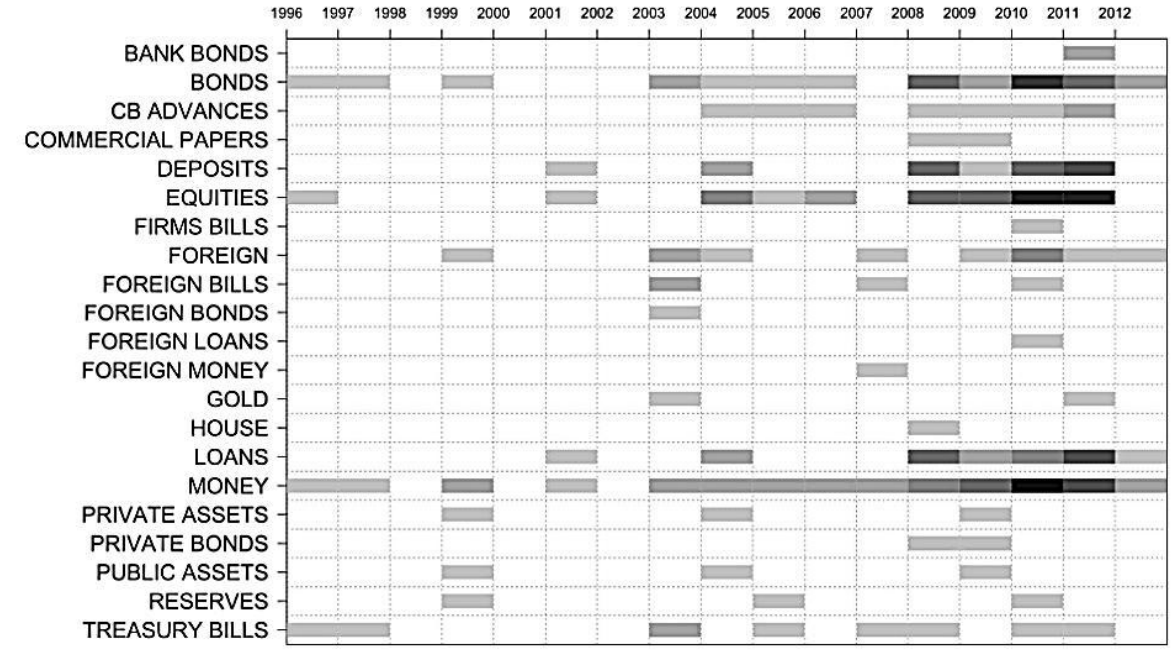
\includegraphics[width = 0.9\textwidth]{./figs/Caverzassi_Heatmap.png}
	\caption*{\textbf{Fonte:} \textcite[p.~4]{caverzasi_stock-flow_2013}}
\end{figure}


Compreendidas tais relações, será desenvolvido um modelo SSM-SFC para dar conta das relações entre lado real e financeiro da economia.
Portanto, esta pesquisa segue o caminho aberto por \textcite{brochier_supermultiplier_2018} ao adicionar um tratamento adequado das relações financeiras no SSM por meio da metodologia SFC estendendo as contribuições de: 
(i) \textcite{jorda_great_2016} ao investigar o processo de ``hipotecarização'' sob um prisma pós-keynesiano a partir de uma análise qualitativa comparativa (QCA); 
%(ii) \textcite{serrano_sraffian_1995} ao incluir o investimento residencial na agenda de pesquisa do supermultiplicador sraffiano; 
(ii) \textcite{teixeira_crescimento_2015} ao avaliar a aplicabilidade da taxa própria de juros dos imóveis para além dos Estados Unidos e;
(iii) \textcite{da_silveira_investimento_2019} ao conectar as relações entre o mercado imobiliário e de crédito diante das especificidades institucionais destacas anteriormente por meio de um modelo SFC de simulação. 




\begin{quote}
	\textit{On the one hand, the German housing
		market was one of the few markets in Western Europe that was not severely affected by the
		global housing boom of the early 2000s. On the other hand, recent developments suggest
		that the role of finance in the German housing system is \textbf{changing}, but not in the same way as
		in other countries}. \cite[p.~969, grifos adicionados]{wijburg_alternative_2017}
\end{quote}

\footnote{Apenas para ilustrar a pluralidade de temas que tal metodologia já abordou, temos --- mesmo que em sua forma mais originária encontrada em \textcite{godley_macroeconomics_1983} --- as formas de financiamento das firmas \cites{asimakopulos_kalecki_1983}{skott_finance_1988}{messori_financing_1991}; endogeneidade da moeda e importância do sistema bancário \cites{messori_financing_1991}{dow_horizontalism:_1996}{arestis_theoretical_1996}{godley_money_1999}; endividamento, distribuição de renda e, apenas para restringir os temas, financeirização \cites{palley_inside_1996}{wolfson_irving_1996}{palley_money_1997}{palley_financial_2002}{dos_santos_revisiting_2009}{palley_inside_2010}{hein_finance-dominated_2012}.}

Sendo assim, o investimento residencial no trabalho de \textcite{nikolaidi_securitisation_2015} possui tanto uma parcela autônoma em relação à renda quanto outra induzida pela renda disponível das famílias.
No entanto, ao partir do procedimento de \textcite{godley_money_1999} para determinação do portfólio de ativos dos agentes, trata os imóveis como um ativo financeiro qualquer sem considerar suas particularidade, qual seja, durabilidade e baixo risco. %TODO: Rever particularidade dos imóveis.


Um  exemplo é o trabalho de  em que são investigados os efeitos da diminuição --- apesar da distribuição da renda a favor dos lucros --- da propensão média a poupar da economia norte-americana por meio da introdução do mercado imobiliário na metodologia SFC\footnote{
	Tal resultado, argumenta, decorre dos ganhos de capital nos mercados imobiliário e acionário entre o topo da distribuição, contribuindo para a diminuição da taxa de poupança.
}. 
Por mais que este trabalho seja uma via para a inclusão do investimento residencial nos modelos macroeconômicos, tal gasto não é o principal determinante da dinâmica  uma vez que parte de uma especificação kaleckiana do investimento das firmas.
Sendo assim, 

Alguns trabalhos seguiram a contribuição de \textcite{zezza_u.s._2008}.
Um deles é o de  com dois tipos de agentes demandando imóveis: parcela dos trabalhadores e investidores institucionais.
Para os primeiros, a demanda por casas é determinada positivamente pela poupança deste setor acrescido de empréstimos hipotecários e negativamente pelo preço dos imóveis de modo que não pode ser considerado estritamente autônomo.
Já os demais agentes, demandam imóveis tal como outros ativos financeiros, ou seja, depende positivamente de sua taxa de retorno.
Em conjunto, tais equações comportamentais determinam que a taxa de crescimento do investimento residencial depende tanto da razão entre a demanda por imóveis em relação ao total quanto de sua inflação que, por sua vez, é determinada pelo estoque de imóveis não vendidos.


%%%%%% ANÁLISE INSTITUCIONAL COMPARATIVA A PARTIR DA NEI -> CHANG: CONFIGURAÇÕES DIFERENTES LEVAM ÀS MESMAS FUNÇÕES. %%%%
A literatura sobre análise institucional comparada se deve, em grande medida, aos desenvolvimentos da Nova Economia Institucional (MENARD e SHIRLEY).
Tal abordagem, no entanto, não faz uma distinção entre formas e funções das instituições além de partir do paradigma ``one-fits-all'' (CHANG 2007, Ch2).
CHANG 2011, por outro lado, argumenta que  diferentes arranjos institucionais podem desempenhar (conjuntamente) as mesmas funções. 
Dito isso, a presente pesquisa parte desta hipótese de ausência de uniformidade causal do arranjo institucional e, assim, enfatizará as particularidades de cada país.



\end{comment}
\section{Plano de trabalho e cronograma de atividades}\label{cronograma}


O trabalho será orientado pelo Prof. Dr. Lucas Azeredo da Silva Teixeira (Unicamp) e coorientado pela Profa. Dra. Ivette Raymunda Luna Huamani (Unicamp). 
A tabela \ref{crono} apresenta um cronograma das atividades. Os capítulos estão destacados em vermelho, as etapas necessárias para concluir cada um deles está em laranja e em cinza as obrigações institucionais.
Cabe destacar que desde o ingresso no programa de doutorado até a
submissão deste projeto, o aluno concluiu as disciplinas necessárias ao cumprimento dos créditos exigidos pelo programa, realizou um estágio de docência, apresentou artigos em congressos
internacionais (\textit{EEA} e \textit{EAEPE}), contribuiu nas atividades do Centro de Estudos de Conjuntura e Política Econômica (Cecon-Unicamp), realizou cursos de R, Python, LSD e QCA (ferramentas a serem utilizadas na pesquisa) e, ao longo do período de avaliação do projeto, submeterá dois artigos referentes à dissertação.
 Como resultado da tese, planeja-se submeter ao menos três artigos para conferências internacionais e nacionais e ao menos três artigos para revistas de circulação internacional indexadas na área.
 %Vale destacar que serão produzidas rotinas e um pacote --- de forma livre e aberta --- para elaboração do modelo fsQCA como subproduto da tese\footnote{Cabe a menção do pacote \textit{fsQCA} em python2 desenvolvido por \textcite{reichert_kirq_2014}. Pretende-se adequar este pacote para python3 e, assim, compatibilizar com os avanços desta linguagem podendo ser estendido para análises de redes sócio-econômicas e redes neurais com \textit{machine learning}.}.

\begin{table}[H]
	\centering
	\caption{Cronograma de atividades}
	\tiny
	\label{crono}
	\resizebox{.7\textwidth}{!}{%
	\begin{tabular}{ll|l|l|l|l|ll}
	\hline\hline
\multicolumn{1}{c}{} & \multicolumn{6}{c}{\textbf{Período}} \\ \cline{2-7} 
\multicolumn{1}{c}{\multirow{-2}{*}{\textbf{Atividades}}} & \multicolumn{1}{c|}{\textbf{1º Semestre 2020}} & \multicolumn{1}{c|}{\textbf{2º Semestre  2020}} & \multicolumn{1}{c|}{\textbf{1º Semestre  2021}} & \multicolumn{1}{c|}{\textbf{2º Semestre  2021}} & \multicolumn{1}{c|}{\textbf{2022}} & \multicolumn{1}{c}{\textbf{2023}} \\ \hline

\textbf{1. Fundamentação teórica} & \cellcolor[HTML]{FF9933} &\cellcolor[HTML]{FF9933}&\cellcolor[HTML]{FF9933}&  & &  \\ \hline
1.1. Disciplinas & \cellcolor[HTML]{9B9B9B} &&&&&  \\ \hline
1.2. Revisão bibliográfica & \cellcolor[HTML]{FF9933} &\cellcolor[HTML]{FF9933}&\cellcolor[HTML]{FF9933}&  & &  \\ \hline

\textbf{2. Modelo QCA} &&\cellcolor[HTML]{FF0000}&\cellcolor[HTML]{FF0000}&\cellcolor[HTML]{FF0000}&& \\ \hline
2.1. Análise comparativa &&\cellcolor[HTML]{FF9933}&\cellcolor[HTML]{FF9933}&\cellcolor[HTML]{FF9933}&& \\ \hline
2.2. Construção e resultados &&&&\cellcolor[HTML]{FF9933}&& \\ \hline

\textbf{3. Qualificação} &&&&\cellcolor[HTML]{9B9B9B}&& \\ \hline

\textbf{4. Modelo Painel} &&\cellcolor[HTML]{FF0000}&\cellcolor[HTML]{FF0000}&\cellcolor[HTML]{FF0000}&\cellcolor[HTML]{FF0000}&\cellcolor[HTML]{FF0000} \\ \hline
4.1. Preparação dos dados &&\cellcolor[HTML]{FF9933}&\cellcolor[HTML]{FF9933}&\cellcolor[HTML]{FF9933}&& \\ \hline
4.2. Estimação e análise &&&&&\cellcolor[HTML]{FF9933}&\cellcolor[HTML]{FF9933} \\ \hline

\textbf{5. Bolsa de Estágio no Exterior (BEPE)}\footnotemark &&&&\cellcolor[HTML]{9B9B9B}&\cellcolor[HTML]{9B9B9B}&\cellcolor[HTML]{9B9B9B}\\ \hline
\textbf{6. Modelo AB-SFC} &&&\cellcolor[HTML]{FF0000}&\cellcolor[HTML]{FF0000}&\cellcolor[HTML]{FF0000}&\cellcolor[HTML]{FF0000} \\ \hline
6.1. Construção &&&\cellcolor[HTML]{FF9933}&\cellcolor[HTML]{FF9933}&& \\ \hline
6.2. Simulação e análise &&&&&\cellcolor[HTML]{FF9933}&\cellcolor[HTML]{FF9933}\\ \hline

\textbf{7. Conclusão e Defesa} & & &  &  & & \cellcolor[HTML]{9B9B9B} \\ \hline \hline
		
	

\end{tabular}%
	\renewcommand{\arraystretch}{0.4}
	}
\caption*{\textbf{Fonte:} Elaboração própria}
\end{table}
\footnotetext{A depender da disponibilidade de financiamento. Está indicado no segundo semestre de 2021 o tempo para reunir documentos e para se preparar para realizar este estágio.}



 
 
\begin{comment}

\end{comment}





\section{Bolsa de estágio no exterior (BEPE)}\label{BEPE}

Pretende-se realizar um estágio no exterior, por meio da BEPE, com duração de 12 meses no segundo semestre de 2022 e
primeiro semestre de 2023 numa instituição de elevado prestígio internacional. Uma opção é a OPÇÃO 1, que conta com
professores renomados que trabalham com a literatura sraffiana, como PROF 1 e
PROF 2. 
\endgroup

%=====================================================================
% 							Bibliografia
%=====================================================================

{
\singlespacing\linespread{0.69}\let\clearpage\relax\printbibliography
}
%=====================================================================
% 							Fim do Documento
%=====================================================================
\end{document}